
    




    
\documentclass[11pt]{article}

    
    \usepackage[breakable]{tcolorbox}
    \tcbset{nobeforeafter} % prevents tcolorboxes being placing in paragraphs
    \usepackage{float}
    \floatplacement{figure}{H} % forces figures to be placed at the correct location
    
    \usepackage[T1]{fontenc}
    % Nicer default font (+ math font) than Computer Modern for most use cases
    \usepackage{mathpazo}

    % Basic figure setup, for now with no caption control since it's done
    % automatically by Pandoc (which extracts ![](path) syntax from Markdown).
    \usepackage{graphicx}
    % We will generate all images so they have a width \maxwidth. This means
    % that they will get their normal width if they fit onto the page, but
    % are scaled down if they would overflow the margins.
    \makeatletter
    \def\maxwidth{\ifdim\Gin@nat@width>\linewidth\linewidth
    \else\Gin@nat@width\fi}
    \makeatother
    \let\Oldincludegraphics\includegraphics
    % Set max figure width to be 80% of text width, for now hardcoded.
    \renewcommand{\includegraphics}[1]{\Oldincludegraphics[width=.8\maxwidth]{#1}}
    % Ensure that by default, figures have no caption (until we provide a
    % proper Figure object with a Caption API and a way to capture that
    % in the conversion process - todo).
    \usepackage{caption}
    \DeclareCaptionLabelFormat{nolabel}{}
    \captionsetup{labelformat=nolabel}

    \usepackage{adjustbox} % Used to constrain images to a maximum size 
    \usepackage{xcolor} % Allow colors to be defined
    \usepackage{enumerate} % Needed for markdown enumerations to work
    \usepackage{geometry} % Used to adjust the document margins
    \usepackage{amsmath} % Equations
    \usepackage{amssymb} % Equations
    \usepackage{textcomp} % defines textquotesingle
    % Hack from http://tex.stackexchange.com/a/47451/13684:
    \AtBeginDocument{%
        \def\PYZsq{\textquotesingle}% Upright quotes in Pygmentized code
    }
    \usepackage{upquote} % Upright quotes for verbatim code
    \usepackage{eurosym} % defines \euro
    \usepackage[mathletters]{ucs} % Extended unicode (utf-8) support
    \usepackage[utf8x]{inputenc} % Allow utf-8 characters in the tex document
    \usepackage{fancyvrb} % verbatim replacement that allows latex
    \usepackage{grffile} % extends the file name processing of package graphics 
                         % to support a larger range 
    % The hyperref package gives us a pdf with properly built
    % internal navigation ('pdf bookmarks' for the table of contents,
    % internal cross-reference links, web links for URLs, etc.)
    \usepackage{hyperref}
    \usepackage{longtable} % longtable support required by pandoc >1.10
    \usepackage{booktabs}  % table support for pandoc > 1.12.2
    \usepackage[inline]{enumitem} % IRkernel/repr support (it uses the enumerate* environment)
    \usepackage[normalem]{ulem} % ulem is needed to support strikethroughs (\sout)
                                % normalem makes italics be italics, not underlines
    \usepackage{mathrsfs}
    

    
    % Colors for the hyperref package
    \definecolor{urlcolor}{rgb}{0,.145,.698}
    \definecolor{linkcolor}{rgb}{.71,0.21,0.01}
    \definecolor{citecolor}{rgb}{.12,.54,.11}

    % ANSI colors
    \definecolor{ansi-black}{HTML}{3E424D}
    \definecolor{ansi-black-intense}{HTML}{282C36}
    \definecolor{ansi-red}{HTML}{E75C58}
    \definecolor{ansi-red-intense}{HTML}{B22B31}
    \definecolor{ansi-green}{HTML}{00A250}
    \definecolor{ansi-green-intense}{HTML}{007427}
    \definecolor{ansi-yellow}{HTML}{DDB62B}
    \definecolor{ansi-yellow-intense}{HTML}{B27D12}
    \definecolor{ansi-blue}{HTML}{208FFB}
    \definecolor{ansi-blue-intense}{HTML}{0065CA}
    \definecolor{ansi-magenta}{HTML}{D160C4}
    \definecolor{ansi-magenta-intense}{HTML}{A03196}
    \definecolor{ansi-cyan}{HTML}{60C6C8}
    \definecolor{ansi-cyan-intense}{HTML}{258F8F}
    \definecolor{ansi-white}{HTML}{C5C1B4}
    \definecolor{ansi-white-intense}{HTML}{A1A6B2}
    \definecolor{ansi-default-inverse-fg}{HTML}{FFFFFF}
    \definecolor{ansi-default-inverse-bg}{HTML}{000000}

    % commands and environments needed by pandoc snippets
    % extracted from the output of `pandoc -s`
    \providecommand{\tightlist}{%
      \setlength{\itemsep}{0pt}\setlength{\parskip}{0pt}}
    \DefineVerbatimEnvironment{Highlighting}{Verbatim}{commandchars=\\\{\}}
    % Add ',fontsize=\small' for more characters per line
    \newenvironment{Shaded}{}{}
    \newcommand{\KeywordTok}[1]{\textcolor[rgb]{0.00,0.44,0.13}{\textbf{{#1}}}}
    \newcommand{\DataTypeTok}[1]{\textcolor[rgb]{0.56,0.13,0.00}{{#1}}}
    \newcommand{\DecValTok}[1]{\textcolor[rgb]{0.25,0.63,0.44}{{#1}}}
    \newcommand{\BaseNTok}[1]{\textcolor[rgb]{0.25,0.63,0.44}{{#1}}}
    \newcommand{\FloatTok}[1]{\textcolor[rgb]{0.25,0.63,0.44}{{#1}}}
    \newcommand{\CharTok}[1]{\textcolor[rgb]{0.25,0.44,0.63}{{#1}}}
    \newcommand{\StringTok}[1]{\textcolor[rgb]{0.25,0.44,0.63}{{#1}}}
    \newcommand{\CommentTok}[1]{\textcolor[rgb]{0.38,0.63,0.69}{\textit{{#1}}}}
    \newcommand{\OtherTok}[1]{\textcolor[rgb]{0.00,0.44,0.13}{{#1}}}
    \newcommand{\AlertTok}[1]{\textcolor[rgb]{1.00,0.00,0.00}{\textbf{{#1}}}}
    \newcommand{\FunctionTok}[1]{\textcolor[rgb]{0.02,0.16,0.49}{{#1}}}
    \newcommand{\RegionMarkerTok}[1]{{#1}}
    \newcommand{\ErrorTok}[1]{\textcolor[rgb]{1.00,0.00,0.00}{\textbf{{#1}}}}
    \newcommand{\NormalTok}[1]{{#1}}
    
    % Additional commands for more recent versions of Pandoc
    \newcommand{\ConstantTok}[1]{\textcolor[rgb]{0.53,0.00,0.00}{{#1}}}
    \newcommand{\SpecialCharTok}[1]{\textcolor[rgb]{0.25,0.44,0.63}{{#1}}}
    \newcommand{\VerbatimStringTok}[1]{\textcolor[rgb]{0.25,0.44,0.63}{{#1}}}
    \newcommand{\SpecialStringTok}[1]{\textcolor[rgb]{0.73,0.40,0.53}{{#1}}}
    \newcommand{\ImportTok}[1]{{#1}}
    \newcommand{\DocumentationTok}[1]{\textcolor[rgb]{0.73,0.13,0.13}{\textit{{#1}}}}
    \newcommand{\AnnotationTok}[1]{\textcolor[rgb]{0.38,0.63,0.69}{\textbf{\textit{{#1}}}}}
    \newcommand{\CommentVarTok}[1]{\textcolor[rgb]{0.38,0.63,0.69}{\textbf{\textit{{#1}}}}}
    \newcommand{\VariableTok}[1]{\textcolor[rgb]{0.10,0.09,0.49}{{#1}}}
    \newcommand{\ControlFlowTok}[1]{\textcolor[rgb]{0.00,0.44,0.13}{\textbf{{#1}}}}
    \newcommand{\OperatorTok}[1]{\textcolor[rgb]{0.40,0.40,0.40}{{#1}}}
    \newcommand{\BuiltInTok}[1]{{#1}}
    \newcommand{\ExtensionTok}[1]{{#1}}
    \newcommand{\PreprocessorTok}[1]{\textcolor[rgb]{0.74,0.48,0.00}{{#1}}}
    \newcommand{\AttributeTok}[1]{\textcolor[rgb]{0.49,0.56,0.16}{{#1}}}
    \newcommand{\InformationTok}[1]{\textcolor[rgb]{0.38,0.63,0.69}{\textbf{\textit{{#1}}}}}
    \newcommand{\WarningTok}[1]{\textcolor[rgb]{0.38,0.63,0.69}{\textbf{\textit{{#1}}}}}
    
    
    % Define a nice break command that doesn't care if a line doesn't already
    % exist.
    \def\br{\hspace*{\fill} \\* }
    % Math Jax compatibility definitions
    \def\gt{>}
    \def\lt{<}
    \let\Oldtex\TeX
    \let\Oldlatex\LaTeX
    \renewcommand{\TeX}{\textrm{\Oldtex}}
    \renewcommand{\LaTeX}{\textrm{\Oldlatex}}
    % Document parameters
    % Document title
    \title{homework\_10\_Yiman Li}
    
    
    
    
    
% Pygments definitions
\makeatletter
\def\PY@reset{\let\PY@it=\relax \let\PY@bf=\relax%
    \let\PY@ul=\relax \let\PY@tc=\relax%
    \let\PY@bc=\relax \let\PY@ff=\relax}
\def\PY@tok#1{\csname PY@tok@#1\endcsname}
\def\PY@toks#1+{\ifx\relax#1\empty\else%
    \PY@tok{#1}\expandafter\PY@toks\fi}
\def\PY@do#1{\PY@bc{\PY@tc{\PY@ul{%
    \PY@it{\PY@bf{\PY@ff{#1}}}}}}}
\def\PY#1#2{\PY@reset\PY@toks#1+\relax+\PY@do{#2}}

\expandafter\def\csname PY@tok@w\endcsname{\def\PY@tc##1{\textcolor[rgb]{0.73,0.73,0.73}{##1}}}
\expandafter\def\csname PY@tok@c\endcsname{\let\PY@it=\textit\def\PY@tc##1{\textcolor[rgb]{0.25,0.50,0.50}{##1}}}
\expandafter\def\csname PY@tok@cp\endcsname{\def\PY@tc##1{\textcolor[rgb]{0.74,0.48,0.00}{##1}}}
\expandafter\def\csname PY@tok@k\endcsname{\let\PY@bf=\textbf\def\PY@tc##1{\textcolor[rgb]{0.00,0.50,0.00}{##1}}}
\expandafter\def\csname PY@tok@kp\endcsname{\def\PY@tc##1{\textcolor[rgb]{0.00,0.50,0.00}{##1}}}
\expandafter\def\csname PY@tok@kt\endcsname{\def\PY@tc##1{\textcolor[rgb]{0.69,0.00,0.25}{##1}}}
\expandafter\def\csname PY@tok@o\endcsname{\def\PY@tc##1{\textcolor[rgb]{0.40,0.40,0.40}{##1}}}
\expandafter\def\csname PY@tok@ow\endcsname{\let\PY@bf=\textbf\def\PY@tc##1{\textcolor[rgb]{0.67,0.13,1.00}{##1}}}
\expandafter\def\csname PY@tok@nb\endcsname{\def\PY@tc##1{\textcolor[rgb]{0.00,0.50,0.00}{##1}}}
\expandafter\def\csname PY@tok@nf\endcsname{\def\PY@tc##1{\textcolor[rgb]{0.00,0.00,1.00}{##1}}}
\expandafter\def\csname PY@tok@nc\endcsname{\let\PY@bf=\textbf\def\PY@tc##1{\textcolor[rgb]{0.00,0.00,1.00}{##1}}}
\expandafter\def\csname PY@tok@nn\endcsname{\let\PY@bf=\textbf\def\PY@tc##1{\textcolor[rgb]{0.00,0.00,1.00}{##1}}}
\expandafter\def\csname PY@tok@ne\endcsname{\let\PY@bf=\textbf\def\PY@tc##1{\textcolor[rgb]{0.82,0.25,0.23}{##1}}}
\expandafter\def\csname PY@tok@nv\endcsname{\def\PY@tc##1{\textcolor[rgb]{0.10,0.09,0.49}{##1}}}
\expandafter\def\csname PY@tok@no\endcsname{\def\PY@tc##1{\textcolor[rgb]{0.53,0.00,0.00}{##1}}}
\expandafter\def\csname PY@tok@nl\endcsname{\def\PY@tc##1{\textcolor[rgb]{0.63,0.63,0.00}{##1}}}
\expandafter\def\csname PY@tok@ni\endcsname{\let\PY@bf=\textbf\def\PY@tc##1{\textcolor[rgb]{0.60,0.60,0.60}{##1}}}
\expandafter\def\csname PY@tok@na\endcsname{\def\PY@tc##1{\textcolor[rgb]{0.49,0.56,0.16}{##1}}}
\expandafter\def\csname PY@tok@nt\endcsname{\let\PY@bf=\textbf\def\PY@tc##1{\textcolor[rgb]{0.00,0.50,0.00}{##1}}}
\expandafter\def\csname PY@tok@nd\endcsname{\def\PY@tc##1{\textcolor[rgb]{0.67,0.13,1.00}{##1}}}
\expandafter\def\csname PY@tok@s\endcsname{\def\PY@tc##1{\textcolor[rgb]{0.73,0.13,0.13}{##1}}}
\expandafter\def\csname PY@tok@sd\endcsname{\let\PY@it=\textit\def\PY@tc##1{\textcolor[rgb]{0.73,0.13,0.13}{##1}}}
\expandafter\def\csname PY@tok@si\endcsname{\let\PY@bf=\textbf\def\PY@tc##1{\textcolor[rgb]{0.73,0.40,0.53}{##1}}}
\expandafter\def\csname PY@tok@se\endcsname{\let\PY@bf=\textbf\def\PY@tc##1{\textcolor[rgb]{0.73,0.40,0.13}{##1}}}
\expandafter\def\csname PY@tok@sr\endcsname{\def\PY@tc##1{\textcolor[rgb]{0.73,0.40,0.53}{##1}}}
\expandafter\def\csname PY@tok@ss\endcsname{\def\PY@tc##1{\textcolor[rgb]{0.10,0.09,0.49}{##1}}}
\expandafter\def\csname PY@tok@sx\endcsname{\def\PY@tc##1{\textcolor[rgb]{0.00,0.50,0.00}{##1}}}
\expandafter\def\csname PY@tok@m\endcsname{\def\PY@tc##1{\textcolor[rgb]{0.40,0.40,0.40}{##1}}}
\expandafter\def\csname PY@tok@gh\endcsname{\let\PY@bf=\textbf\def\PY@tc##1{\textcolor[rgb]{0.00,0.00,0.50}{##1}}}
\expandafter\def\csname PY@tok@gu\endcsname{\let\PY@bf=\textbf\def\PY@tc##1{\textcolor[rgb]{0.50,0.00,0.50}{##1}}}
\expandafter\def\csname PY@tok@gd\endcsname{\def\PY@tc##1{\textcolor[rgb]{0.63,0.00,0.00}{##1}}}
\expandafter\def\csname PY@tok@gi\endcsname{\def\PY@tc##1{\textcolor[rgb]{0.00,0.63,0.00}{##1}}}
\expandafter\def\csname PY@tok@gr\endcsname{\def\PY@tc##1{\textcolor[rgb]{1.00,0.00,0.00}{##1}}}
\expandafter\def\csname PY@tok@ge\endcsname{\let\PY@it=\textit}
\expandafter\def\csname PY@tok@gs\endcsname{\let\PY@bf=\textbf}
\expandafter\def\csname PY@tok@gp\endcsname{\let\PY@bf=\textbf\def\PY@tc##1{\textcolor[rgb]{0.00,0.00,0.50}{##1}}}
\expandafter\def\csname PY@tok@go\endcsname{\def\PY@tc##1{\textcolor[rgb]{0.53,0.53,0.53}{##1}}}
\expandafter\def\csname PY@tok@gt\endcsname{\def\PY@tc##1{\textcolor[rgb]{0.00,0.27,0.87}{##1}}}
\expandafter\def\csname PY@tok@err\endcsname{\def\PY@bc##1{\setlength{\fboxsep}{0pt}\fcolorbox[rgb]{1.00,0.00,0.00}{1,1,1}{\strut ##1}}}
\expandafter\def\csname PY@tok@kc\endcsname{\let\PY@bf=\textbf\def\PY@tc##1{\textcolor[rgb]{0.00,0.50,0.00}{##1}}}
\expandafter\def\csname PY@tok@kd\endcsname{\let\PY@bf=\textbf\def\PY@tc##1{\textcolor[rgb]{0.00,0.50,0.00}{##1}}}
\expandafter\def\csname PY@tok@kn\endcsname{\let\PY@bf=\textbf\def\PY@tc##1{\textcolor[rgb]{0.00,0.50,0.00}{##1}}}
\expandafter\def\csname PY@tok@kr\endcsname{\let\PY@bf=\textbf\def\PY@tc##1{\textcolor[rgb]{0.00,0.50,0.00}{##1}}}
\expandafter\def\csname PY@tok@bp\endcsname{\def\PY@tc##1{\textcolor[rgb]{0.00,0.50,0.00}{##1}}}
\expandafter\def\csname PY@tok@fm\endcsname{\def\PY@tc##1{\textcolor[rgb]{0.00,0.00,1.00}{##1}}}
\expandafter\def\csname PY@tok@vc\endcsname{\def\PY@tc##1{\textcolor[rgb]{0.10,0.09,0.49}{##1}}}
\expandafter\def\csname PY@tok@vg\endcsname{\def\PY@tc##1{\textcolor[rgb]{0.10,0.09,0.49}{##1}}}
\expandafter\def\csname PY@tok@vi\endcsname{\def\PY@tc##1{\textcolor[rgb]{0.10,0.09,0.49}{##1}}}
\expandafter\def\csname PY@tok@vm\endcsname{\def\PY@tc##1{\textcolor[rgb]{0.10,0.09,0.49}{##1}}}
\expandafter\def\csname PY@tok@sa\endcsname{\def\PY@tc##1{\textcolor[rgb]{0.73,0.13,0.13}{##1}}}
\expandafter\def\csname PY@tok@sb\endcsname{\def\PY@tc##1{\textcolor[rgb]{0.73,0.13,0.13}{##1}}}
\expandafter\def\csname PY@tok@sc\endcsname{\def\PY@tc##1{\textcolor[rgb]{0.73,0.13,0.13}{##1}}}
\expandafter\def\csname PY@tok@dl\endcsname{\def\PY@tc##1{\textcolor[rgb]{0.73,0.13,0.13}{##1}}}
\expandafter\def\csname PY@tok@s2\endcsname{\def\PY@tc##1{\textcolor[rgb]{0.73,0.13,0.13}{##1}}}
\expandafter\def\csname PY@tok@sh\endcsname{\def\PY@tc##1{\textcolor[rgb]{0.73,0.13,0.13}{##1}}}
\expandafter\def\csname PY@tok@s1\endcsname{\def\PY@tc##1{\textcolor[rgb]{0.73,0.13,0.13}{##1}}}
\expandafter\def\csname PY@tok@mb\endcsname{\def\PY@tc##1{\textcolor[rgb]{0.40,0.40,0.40}{##1}}}
\expandafter\def\csname PY@tok@mf\endcsname{\def\PY@tc##1{\textcolor[rgb]{0.40,0.40,0.40}{##1}}}
\expandafter\def\csname PY@tok@mh\endcsname{\def\PY@tc##1{\textcolor[rgb]{0.40,0.40,0.40}{##1}}}
\expandafter\def\csname PY@tok@mi\endcsname{\def\PY@tc##1{\textcolor[rgb]{0.40,0.40,0.40}{##1}}}
\expandafter\def\csname PY@tok@il\endcsname{\def\PY@tc##1{\textcolor[rgb]{0.40,0.40,0.40}{##1}}}
\expandafter\def\csname PY@tok@mo\endcsname{\def\PY@tc##1{\textcolor[rgb]{0.40,0.40,0.40}{##1}}}
\expandafter\def\csname PY@tok@ch\endcsname{\let\PY@it=\textit\def\PY@tc##1{\textcolor[rgb]{0.25,0.50,0.50}{##1}}}
\expandafter\def\csname PY@tok@cm\endcsname{\let\PY@it=\textit\def\PY@tc##1{\textcolor[rgb]{0.25,0.50,0.50}{##1}}}
\expandafter\def\csname PY@tok@cpf\endcsname{\let\PY@it=\textit\def\PY@tc##1{\textcolor[rgb]{0.25,0.50,0.50}{##1}}}
\expandafter\def\csname PY@tok@c1\endcsname{\let\PY@it=\textit\def\PY@tc##1{\textcolor[rgb]{0.25,0.50,0.50}{##1}}}
\expandafter\def\csname PY@tok@cs\endcsname{\let\PY@it=\textit\def\PY@tc##1{\textcolor[rgb]{0.25,0.50,0.50}{##1}}}

\def\PYZbs{\char`\\}
\def\PYZus{\char`\_}
\def\PYZob{\char`\{}
\def\PYZcb{\char`\}}
\def\PYZca{\char`\^}
\def\PYZam{\char`\&}
\def\PYZlt{\char`\<}
\def\PYZgt{\char`\>}
\def\PYZsh{\char`\#}
\def\PYZpc{\char`\%}
\def\PYZdl{\char`\$}
\def\PYZhy{\char`\-}
\def\PYZsq{\char`\'}
\def\PYZdq{\char`\"}
\def\PYZti{\char`\~}
% for compatibility with earlier versions
\def\PYZat{@}
\def\PYZlb{[}
\def\PYZrb{]}
\makeatother


    % For linebreaks inside Verbatim environment from package fancyvrb. 
    \makeatletter
        \newbox\Wrappedcontinuationbox 
        \newbox\Wrappedvisiblespacebox 
        \newcommand*\Wrappedvisiblespace {\textcolor{red}{\textvisiblespace}} 
        \newcommand*\Wrappedcontinuationsymbol {\textcolor{red}{\llap{\tiny$\m@th\hookrightarrow$}}} 
        \newcommand*\Wrappedcontinuationindent {3ex } 
        \newcommand*\Wrappedafterbreak {\kern\Wrappedcontinuationindent\copy\Wrappedcontinuationbox} 
        % Take advantage of the already applied Pygments mark-up to insert 
        % potential linebreaks for TeX processing. 
        %        {, <, #, %, $, ' and ": go to next line. 
        %        _, }, ^, &, >, - and ~: stay at end of broken line. 
        % Use of \textquotesingle for straight quote. 
        \newcommand*\Wrappedbreaksatspecials {% 
            \def\PYGZus{\discretionary{\char`\_}{\Wrappedafterbreak}{\char`\_}}% 
            \def\PYGZob{\discretionary{}{\Wrappedafterbreak\char`\{}{\char`\{}}% 
            \def\PYGZcb{\discretionary{\char`\}}{\Wrappedafterbreak}{\char`\}}}% 
            \def\PYGZca{\discretionary{\char`\^}{\Wrappedafterbreak}{\char`\^}}% 
            \def\PYGZam{\discretionary{\char`\&}{\Wrappedafterbreak}{\char`\&}}% 
            \def\PYGZlt{\discretionary{}{\Wrappedafterbreak\char`\<}{\char`\<}}% 
            \def\PYGZgt{\discretionary{\char`\>}{\Wrappedafterbreak}{\char`\>}}% 
            \def\PYGZsh{\discretionary{}{\Wrappedafterbreak\char`\#}{\char`\#}}% 
            \def\PYGZpc{\discretionary{}{\Wrappedafterbreak\char`\%}{\char`\%}}% 
            \def\PYGZdl{\discretionary{}{\Wrappedafterbreak\char`\$}{\char`\$}}% 
            \def\PYGZhy{\discretionary{\char`\-}{\Wrappedafterbreak}{\char`\-}}% 
            \def\PYGZsq{\discretionary{}{\Wrappedafterbreak\textquotesingle}{\textquotesingle}}% 
            \def\PYGZdq{\discretionary{}{\Wrappedafterbreak\char`\"}{\char`\"}}% 
            \def\PYGZti{\discretionary{\char`\~}{\Wrappedafterbreak}{\char`\~}}% 
        } 
        % Some characters . , ; ? ! / are not pygmentized. 
        % This macro makes them "active" and they will insert potential linebreaks 
        \newcommand*\Wrappedbreaksatpunct {% 
            \lccode`\~`\.\lowercase{\def~}{\discretionary{\hbox{\char`\.}}{\Wrappedafterbreak}{\hbox{\char`\.}}}% 
            \lccode`\~`\,\lowercase{\def~}{\discretionary{\hbox{\char`\,}}{\Wrappedafterbreak}{\hbox{\char`\,}}}% 
            \lccode`\~`\;\lowercase{\def~}{\discretionary{\hbox{\char`\;}}{\Wrappedafterbreak}{\hbox{\char`\;}}}% 
            \lccode`\~`\:\lowercase{\def~}{\discretionary{\hbox{\char`\:}}{\Wrappedafterbreak}{\hbox{\char`\:}}}% 
            \lccode`\~`\?\lowercase{\def~}{\discretionary{\hbox{\char`\?}}{\Wrappedafterbreak}{\hbox{\char`\?}}}% 
            \lccode`\~`\!\lowercase{\def~}{\discretionary{\hbox{\char`\!}}{\Wrappedafterbreak}{\hbox{\char`\!}}}% 
            \lccode`\~`\/\lowercase{\def~}{\discretionary{\hbox{\char`\/}}{\Wrappedafterbreak}{\hbox{\char`\/}}}% 
            \catcode`\.\active
            \catcode`\,\active 
            \catcode`\;\active
            \catcode`\:\active
            \catcode`\?\active
            \catcode`\!\active
            \catcode`\/\active 
            \lccode`\~`\~ 	
        }
    \makeatother

    \let\OriginalVerbatim=\Verbatim
    \makeatletter
    \renewcommand{\Verbatim}[1][1]{%
        %\parskip\z@skip
        \sbox\Wrappedcontinuationbox {\Wrappedcontinuationsymbol}%
        \sbox\Wrappedvisiblespacebox {\FV@SetupFont\Wrappedvisiblespace}%
        \def\FancyVerbFormatLine ##1{\hsize\linewidth
            \vtop{\raggedright\hyphenpenalty\z@\exhyphenpenalty\z@
                \doublehyphendemerits\z@\finalhyphendemerits\z@
                \strut ##1\strut}%
        }%
        % If the linebreak is at a space, the latter will be displayed as visible
        % space at end of first line, and a continuation symbol starts next line.
        % Stretch/shrink are however usually zero for typewriter font.
        \def\FV@Space {%
            \nobreak\hskip\z@ plus\fontdimen3\font minus\fontdimen4\font
            \discretionary{\copy\Wrappedvisiblespacebox}{\Wrappedafterbreak}
            {\kern\fontdimen2\font}%
        }%
        
        % Allow breaks at special characters using \PYG... macros.
        \Wrappedbreaksatspecials
        % Breaks at punctuation characters . , ; ? ! and / need catcode=\active 	
        \OriginalVerbatim[#1,codes*=\Wrappedbreaksatpunct]%
    }
    \makeatother

    % Exact colors from NB
    \definecolor{incolor}{HTML}{303F9F}
    \definecolor{outcolor}{HTML}{D84315}
    \definecolor{cellborder}{HTML}{CFCFCF}
    \definecolor{cellbackground}{HTML}{F7F7F7}
    
    % prompt
    \newcommand{\prompt}[4]{
        \llap{{\color{#2}[#3]: #4}}\vspace{-1.25em}
    }
    

    
    % Prevent overflowing lines due to hard-to-break entities
    \sloppy 
    % Setup hyperref package
    \hypersetup{
      breaklinks=true,  % so long urls are correctly broken across lines
      colorlinks=true,
      urlcolor=urlcolor,
      linkcolor=linkcolor,
      citecolor=citecolor,
      }
    % Slightly bigger margins than the latex defaults
    
    \geometry{verbose,tmargin=1in,bmargin=1in,lmargin=1in,rmargin=1in}
    
    

    \begin{document}
    
    
    \maketitle
    
    

    
    \begin{tcolorbox}[breakable, size=fbox, boxrule=1pt, pad at break*=1mm,colback=cellbackground, colframe=cellborder]
\prompt{In}{incolor}{1}{\hspace{4pt}}
\begin{Verbatim}[commandchars=\\\{\}]
\PY{k+kn}{import} \PY{n+nn}{copy}
\PY{k+kn}{import} \PY{n+nn}{numpy} \PY{k}{as} \PY{n+nn}{np}
\PY{k+kn}{import} \PY{n+nn}{torch}
\PY{k+kn}{import} \PY{n+nn}{torch}\PY{n+nn}{.}\PY{n+nn}{nn} \PY{k}{as} \PY{n+nn}{nn}
\PY{k+kn}{import} \PY{n+nn}{torch}\PY{n+nn}{.}\PY{n+nn}{nn}\PY{n+nn}{.}\PY{n+nn}{functional} \PY{k}{as} \PY{n+nn}{F}
\PY{k+kn}{import} \PY{n+nn}{torchvision}
\PY{k+kn}{import} \PY{n+nn}{torchvision}\PY{n+nn}{.}\PY{n+nn}{transforms} \PY{k}{as} \PY{n+nn}{transforms}
\end{Verbatim}
\end{tcolorbox}

    \hypertarget{pytorch}{%
\section{PyTorch}\label{pytorch}}

In this notebook you will gain some hands-on experience with
\href{https://pytorch.org/}{PyTorch}, one of the major frameworks for
deep learning. To install PyTorch run
\texttt{conda\ install\ pytorch\ torchvision\ cudatoolkit=10.1\ -c\ pytorch},
with cudatoolkit set to whichever CUDA version you have installed. You
can check this by running \texttt{nvcc\ -\/-version}. If you do not have
an Nvidia GPU you can run
\texttt{conda\ install\ pytorch\ torchvision\ cpuonly\ -c\ pytorch}
instead. However, in this case we recommend using
\href{https://colab.research.google.com/}{Google Colab}.

You will start by re-implementing some common features of deep neural
networks (dropout and batch normalization) and then implement a very
popular modern architecture for image classification (ResNet) and
improve its training loop.

    \hypertarget{dropout}{%
\section{1. Dropout}\label{dropout}}

Dropout is a form of regularization for neural networks. It works by
randomly setting activations (values) to 0, each one with equal
probability \texttt{p}. The values are then scaled by a factor
\(\frac{1}{1-p}\) to conserve their mean.

Dropout effectively trains a pseudo-ensemble of models with stochastic
gradient descent. During evaluation we want to use the full ensemble and
therefore have to turn off dropout. Use \texttt{self.training} to check
if the model is in training or evaluation mode.

Do not use any dropout implementation from PyTorch for this!

    \begin{tcolorbox}[breakable, size=fbox, boxrule=1pt, pad at break*=1mm,colback=cellbackground, colframe=cellborder]
\prompt{In}{incolor}{2}{\hspace{4pt}}
\begin{Verbatim}[commandchars=\\\{\}]
\PY{k}{class} \PY{n+nc}{Dropout}\PY{p}{(}\PY{n}{nn}\PY{o}{.}\PY{n}{Module}\PY{p}{)}\PY{p}{:}
    \PY{l+s+sd}{\PYZdq{}\PYZdq{}\PYZdq{}}
\PY{l+s+sd}{    Dropout, as discussed in the lecture and described here:}
\PY{l+s+sd}{    https://pytorch.org/docs/stable/nn.html\PYZsh{}torch.nn.Dropout}
\PY{l+s+sd}{    }
\PY{l+s+sd}{    Args:}
\PY{l+s+sd}{        p: float, dropout probability}
\PY{l+s+sd}{    \PYZdq{}\PYZdq{}\PYZdq{}}
    \PY{k}{def} \PY{n+nf}{\PYZus{}\PYZus{}init\PYZus{}\PYZus{}}\PY{p}{(}\PY{n+nb+bp}{self}\PY{p}{,} \PY{n}{p}\PY{p}{)}\PY{p}{:}
        \PY{n+nb}{super}\PY{p}{(}\PY{p}{)}\PY{o}{.}\PY{n+nf+fm}{\PYZus{}\PYZus{}init\PYZus{}\PYZus{}}\PY{p}{(}\PY{p}{)}
        \PY{n+nb+bp}{self}\PY{o}{.}\PY{n}{p} \PY{o}{=} \PY{n}{p}
        
    \PY{k}{def} \PY{n+nf}{forward}\PY{p}{(}\PY{n+nb+bp}{self}\PY{p}{,} \PY{n+nb}{input}\PY{p}{)}\PY{p}{:}
        \PY{l+s+sd}{\PYZdq{}\PYZdq{}\PYZdq{}}
\PY{l+s+sd}{        The module\PYZsq{}s forward pass.}
\PY{l+s+sd}{        This has to be implemented for every PyTorch module.}
\PY{l+s+sd}{        PyTorch then automatically generates the backward pass}
\PY{l+s+sd}{        by dynamically generating the computational graph during}
\PY{l+s+sd}{        execution.}
\PY{l+s+sd}{        }
\PY{l+s+sd}{        Args:}
\PY{l+s+sd}{            input: PyTorch tensor, arbitrary shape}

\PY{l+s+sd}{        Returns:}
\PY{l+s+sd}{            PyTorch tensor, same shape as input}
\PY{l+s+sd}{        \PYZdq{}\PYZdq{}\PYZdq{}}
        
         \PY{c+c1}{\PYZsh{} TODO: Set values randomly to 0.}
        \PY{n}{drop\PYZus{}prob} \PY{o}{=} \PY{n+nb+bp}{self}\PY{o}{.}\PY{n}{p}
        \PY{n}{keep\PYZus{}prob} \PY{o}{=} \PY{l+m+mi}{1} \PY{o}{\PYZhy{}} \PY{n}{drop\PYZus{}prob}
        \PY{k}{if} \PY{n}{keep\PYZus{}prob}\PY{o}{==}\PY{l+m+mi}{0}\PY{p}{:}
            \PY{k}{return} \PY{n}{torch}\PY{o}{.}\PY{n}{zeros\PYZus{}like}\PY{p}{(}\PY{n+nb}{input}\PY{p}{)}
        \PY{n}{sample} \PY{o}{=} \PY{n}{torch}\PY{o}{.}\PY{n}{rand}\PY{p}{(}\PY{n+nb}{input}\PY{o}{.}\PY{n}{shape}\PY{p}{)} \PY{o}{\PYZlt{}} \PY{n}{keep\PYZus{}prob}
        \PY{k}{return} \PY{n}{sample} \PY{o}{*} \PY{n+nb}{input} \PY{o}{/} \PY{n}{keep\PYZus{}prob}
\end{Verbatim}
\end{tcolorbox}

    \begin{tcolorbox}[breakable, size=fbox, boxrule=1pt, pad at break*=1mm,colback=cellbackground, colframe=cellborder]
\prompt{In}{incolor}{3}{\hspace{4pt}}
\begin{Verbatim}[commandchars=\\\{\}]
\PY{c+c1}{\PYZsh{} Test dropout}
\PY{n}{test} \PY{o}{=} \PY{n}{torch}\PY{o}{.}\PY{n}{ones}\PY{p}{(}\PY{l+m+mi}{10\PYZus{}000}\PY{p}{)}
\PY{n}{dropout} \PY{o}{=} \PY{n}{Dropout}\PY{p}{(}\PY{l+m+mf}{0.5}\PY{p}{)}
\PY{n}{test\PYZus{}dropped} \PY{o}{=} \PY{n}{dropout}\PY{p}{(}\PY{n}{test}\PY{p}{)}

\PY{c+c1}{\PYZsh{} These assertions can in principle fail due to bad luck, but}
\PY{c+c1}{\PYZsh{} if implemented correctly they should almost always succeed.}
\PY{k}{assert} \PY{n}{np}\PY{o}{.}\PY{n}{isclose}\PY{p}{(}\PY{n}{test\PYZus{}dropped}\PY{o}{.}\PY{n}{sum}\PY{p}{(}\PY{p}{)}\PY{o}{.}\PY{n}{item}\PY{p}{(}\PY{p}{)}\PY{p}{,} \PY{l+m+mi}{10\PYZus{}000}\PY{p}{,} \PY{n}{atol}\PY{o}{=}\PY{l+m+mi}{400}\PY{p}{)}
\PY{k}{assert} \PY{n}{np}\PY{o}{.}\PY{n}{isclose}\PY{p}{(}\PY{p}{(}\PY{n}{test\PYZus{}dropped} \PY{o}{\PYZgt{}} \PY{l+m+mi}{0}\PY{p}{)}\PY{o}{.}\PY{n}{sum}\PY{p}{(}\PY{p}{)}\PY{o}{.}\PY{n}{item}\PY{p}{(}\PY{p}{)}\PY{p}{,} \PY{l+m+mi}{5\PYZus{}000}\PY{p}{,} \PY{n}{atol}\PY{o}{=}\PY{l+m+mi}{200}\PY{p}{)}
\end{Verbatim}
\end{tcolorbox}

    \hypertarget{batch-normalization}{%
\section{2. Batch normalization}\label{batch-normalization}}

Batch normalization is a trick use to smoothen the loss landscape and
improve training. It is defined as the function
\[y = \frac{x - \mu_x}{\sigma_x + \epsilon} \cdot \gamma + \beta\],
where \(\gamma\) and \(\beta\) and learnable parameters and \(\epsilon\)
is a some small number to avoid dividing by zero. The Statistics
\(\mu_x\) and \(\sigma_x\) are taken separately for each feature. In a
CNN this means averaging over the batch and all pixels.

Do not use any batch normalization implementation from PyTorch for this!

    \begin{tcolorbox}[breakable, size=fbox, boxrule=1pt, pad at break*=1mm,colback=cellbackground, colframe=cellborder]
\prompt{In}{incolor}{4}{\hspace{4pt}}
\begin{Verbatim}[commandchars=\\\{\}]
\PY{k}{class} \PY{n+nc}{BatchNorm}\PY{p}{(}\PY{n}{nn}\PY{o}{.}\PY{n}{Module}\PY{p}{)}\PY{p}{:}
    \PY{l+s+sd}{\PYZdq{}\PYZdq{}\PYZdq{}}
\PY{l+s+sd}{    Batch normalization, as discussed in the lecture and similar to}
\PY{l+s+sd}{    https://pytorch.org/docs/stable/nn.html\PYZsh{}torch.nn.BatchNorm1d}
\PY{l+s+sd}{    }
\PY{l+s+sd}{    Only uses batch statistics (no running mean for evaluation).}
\PY{l+s+sd}{    Batch statistics are calculated for a single dimension.}
\PY{l+s+sd}{    Gamma is initialized as 1, beta as 0.}
\PY{l+s+sd}{    }
\PY{l+s+sd}{    Args:}
\PY{l+s+sd}{        num\PYZus{}features: Number of features to calculate batch statistics for.}
\PY{l+s+sd}{    \PYZdq{}\PYZdq{}\PYZdq{}}
    \PY{k}{def} \PY{n+nf}{\PYZus{}\PYZus{}init\PYZus{}\PYZus{}}\PY{p}{(}\PY{n+nb+bp}{self}\PY{p}{,} \PY{n}{num\PYZus{}features}\PY{p}{)}\PY{p}{:}
        \PY{n+nb}{super}\PY{p}{(}\PY{p}{)}\PY{o}{.}\PY{n+nf+fm}{\PYZus{}\PYZus{}init\PYZus{}\PYZus{}}\PY{p}{(}\PY{p}{)}
        
        \PY{c+c1}{\PYZsh{} TODO: Initialize the required parameters}
        \PY{n+nb+bp}{self}\PY{o}{.}\PY{n}{gamma} \PY{o}{=} \PY{n}{nn}\PY{o}{.}\PY{n}{Parameter}\PY{p}{(}\PY{n}{torch}\PY{o}{.}\PY{n}{ones}\PY{p}{(}\PY{n}{num\PYZus{}features}\PY{p}{)}\PY{p}{)}
        \PY{n+nb+bp}{self}\PY{o}{.}\PY{n}{beta} \PY{o}{=} \PY{n}{nn}\PY{o}{.}\PY{n}{Parameter}\PY{p}{(}\PY{n}{torch}\PY{o}{.}\PY{n}{zeros}\PY{p}{(}\PY{n}{num\PYZus{}features}\PY{p}{)}\PY{p}{)}
        
    \PY{k}{def} \PY{n+nf}{forward}\PY{p}{(}\PY{n+nb+bp}{self}\PY{p}{,} \PY{n+nb}{input}\PY{p}{)}\PY{p}{:}
        \PY{l+s+sd}{\PYZdq{}\PYZdq{}\PYZdq{}}
\PY{l+s+sd}{        Batch normalization over the dimension C of (N, C, L).}
\PY{l+s+sd}{        }
\PY{l+s+sd}{        Args:}
\PY{l+s+sd}{            input: PyTorch tensor, shape [N, C, L]}
\PY{l+s+sd}{            }
\PY{l+s+sd}{        Return:}
\PY{l+s+sd}{            PyTorch tensor, same shape as input}
\PY{l+s+sd}{        \PYZdq{}\PYZdq{}\PYZdq{}}
        \PY{n}{eps} \PY{o}{=} \PY{l+m+mf}{1e\PYZhy{}5}
        
        \PY{c+c1}{\PYZsh{} TODO: Implement the required transformation}
        \PY{n}{N}\PY{p}{,} \PY{n}{C}\PY{p}{,} \PY{n}{L} \PY{o}{=} \PY{n+nb}{input}\PY{o}{.}\PY{n}{shape}
        \PY{n}{gamma} \PY{o}{=} \PY{n+nb+bp}{self}\PY{o}{.}\PY{n}{gamma}\PY{o}{.}\PY{n}{unsqueeze}\PY{p}{(}\PY{l+m+mi}{0}\PY{p}{)}\PY{o}{.}\PY{n}{unsqueeze}\PY{p}{(}\PY{o}{\PYZhy{}}\PY{l+m+mi}{1}\PY{p}{)}\PY{o}{.}\PY{n}{expand}\PY{p}{(}\PY{n}{N}\PY{p}{,} \PY{n}{C}\PY{p}{,} \PY{n}{L}\PY{p}{)}
        \PY{n}{beta} \PY{o}{=} \PY{n+nb+bp}{self}\PY{o}{.}\PY{n}{beta}\PY{o}{.}\PY{n}{unsqueeze}\PY{p}{(}\PY{l+m+mi}{0}\PY{p}{)}\PY{o}{.}\PY{n}{unsqueeze}\PY{p}{(}\PY{o}{\PYZhy{}}\PY{l+m+mi}{1}\PY{p}{)}\PY{o}{.}\PY{n}{expand}\PY{p}{(}\PY{n}{N}\PY{p}{,} \PY{n}{C}\PY{p}{,} \PY{n}{L}\PY{p}{)}
        
        \PY{n}{x} \PY{o}{=} \PY{n+nb}{input}\PY{p}{[}\PY{l+m+mi}{0}\PY{p}{]}
        \PY{k}{for} \PY{n}{i} \PY{o+ow}{in} \PY{n+nb}{range}\PY{p}{(}\PY{n}{N}\PY{o}{\PYZhy{}}\PY{l+m+mi}{1}\PY{p}{)}\PY{p}{:}
            \PY{n}{x} \PY{o}{=} \PY{n}{torch}\PY{o}{.}\PY{n}{cat}\PY{p}{(}\PY{p}{(}\PY{n}{x}\PY{p}{,} \PY{n+nb}{input}\PY{p}{[}\PY{n}{i}\PY{o}{+}\PY{l+m+mi}{1}\PY{p}{]}\PY{p}{)}\PY{p}{,} \PY{n}{dim}\PY{o}{=}\PY{l+m+mi}{1}\PY{p}{)}
        
        \PY{n}{mean\PYZus{}x} \PY{o}{=} \PY{p}{(}\PY{n}{x}\PY{o}{.}\PY{n}{mean}\PY{p}{(}\PY{n}{axis}\PY{o}{=}\PY{l+m+mi}{1}\PY{p}{)}\PY{o}{.}\PY{n}{unsqueeze}\PY{p}{(}\PY{l+m+mi}{0}\PY{p}{)}\PY{p}{)}\PY{o}{.}\PY{n}{unsqueeze}\PY{p}{(}\PY{o}{\PYZhy{}}\PY{l+m+mi}{1}\PY{p}{)}\PY{o}{.}\PY{n}{expand}\PY{p}{(}\PY{n}{N}\PY{p}{,} \PY{n}{C}\PY{p}{,} \PY{n}{L}\PY{p}{)}  \PY{c+c1}{\PYZsh{}TensorSize([N,C,L])}
              
        \PY{n}{var} \PY{o}{=} \PY{n}{x}\PY{o}{.}\PY{n}{var}\PY{p}{(}\PY{n}{axis} \PY{o}{=} \PY{l+m+mi}{1}\PY{p}{)} \PY{o}{*} \PY{p}{(}\PY{n}{N}\PY{o}{*}\PY{n}{L}\PY{o}{\PYZhy{}}\PY{l+m+mi}{1}\PY{p}{)} \PY{o}{/} \PY{p}{(}\PY{n}{N}\PY{o}{*}\PY{n}{L}\PY{p}{)} \PY{c+c1}{\PYZsh{} TensorSize([C])}
        \PY{n}{sta\PYZus{}x} \PY{o}{=} \PY{n}{torch}\PY{o}{.}\PY{n}{sqrt}\PY{p}{(}\PY{p}{(}\PY{n}{var}\PY{o}{.}\PY{n}{unsqueeze}\PY{p}{(}\PY{l+m+mi}{0}\PY{p}{)}\PY{p}{)}\PY{o}{.}\PY{n}{unsqueeze}\PY{p}{(}\PY{o}{\PYZhy{}}\PY{l+m+mi}{1}\PY{p}{)}\PY{o}{.}\PY{n}{expand}\PY{p}{(}\PY{n}{N}\PY{p}{,} \PY{n}{C}\PY{p}{,} \PY{n}{L}\PY{p}{)}\PY{p}{)}
        
        \PY{n}{x\PYZus{}normalize} \PY{o}{=} \PY{p}{(}\PY{n+nb}{input} \PY{o}{\PYZhy{}} \PY{n}{mean\PYZus{}x}\PY{p}{)} \PY{o}{/} \PY{p}{(}\PY{n}{sta\PYZus{}x} \PY{o}{+} \PY{n}{eps}\PY{p}{)}
        \PY{n}{x\PYZus{}scale} \PY{o}{=} \PY{n}{x\PYZus{}normalize} \PY{o}{*} \PY{n}{gamma} \PY{o}{+} \PY{n}{beta}
        
        \PY{k}{return} \PY{n}{x\PYZus{}scale}
\end{Verbatim}
\end{tcolorbox}

    \begin{tcolorbox}[breakable, size=fbox, boxrule=1pt, pad at break*=1mm,colback=cellbackground, colframe=cellborder]
\prompt{In}{incolor}{5}{\hspace{4pt}}
\begin{Verbatim}[commandchars=\\\{\}]
\PY{c+c1}{\PYZsh{} Tests the batch normalization implementation}
\PY{n}{torch}\PY{o}{.}\PY{n}{random}\PY{o}{.}\PY{n}{manual\PYZus{}seed}\PY{p}{(}\PY{l+m+mi}{42}\PY{p}{)}
\PY{n}{test} \PY{o}{=} \PY{n}{torch}\PY{o}{.}\PY{n}{randn}\PY{p}{(}\PY{l+m+mi}{8}\PY{p}{,} \PY{l+m+mi}{2}\PY{p}{,} \PY{l+m+mi}{4}\PY{p}{)}

\PY{n}{b1} \PY{o}{=} \PY{n}{BatchNorm}\PY{p}{(}\PY{l+m+mi}{2}\PY{p}{)}
\PY{n}{test\PYZus{}b1} \PY{o}{=} \PY{n}{b1}\PY{p}{(}\PY{n}{test}\PY{p}{)}

\PY{n}{b2} \PY{o}{=} \PY{n}{nn}\PY{o}{.}\PY{n}{BatchNorm1d}\PY{p}{(}\PY{l+m+mi}{2}\PY{p}{,} \PY{n}{affine}\PY{o}{=}\PY{k+kc}{False}\PY{p}{,} \PY{n}{track\PYZus{}running\PYZus{}stats}\PY{o}{=}\PY{k+kc}{False}\PY{p}{)}
\PY{n}{test\PYZus{}b2} \PY{o}{=} \PY{n}{b2}\PY{p}{(}\PY{n}{test}\PY{p}{)}

\PY{k}{assert} \PY{n}{torch}\PY{o}{.}\PY{n}{allclose}\PY{p}{(}\PY{n}{test\PYZus{}b1}\PY{p}{,} \PY{n}{test\PYZus{}b2}\PY{p}{,} \PY{n}{rtol}\PY{o}{=}\PY{l+m+mf}{0.02}\PY{p}{)}
\end{Verbatim}
\end{tcolorbox}

    \hypertarget{resnet}{%
\section{3. ResNet}\label{resnet}}

ResNet is the models that first introduced residual connections (a form
of skip connections). It is a rather simple, but successful and very
popular architecture. In this part of the exercise we will re-implement
it step by step.

Note that there is also an
\href{https://arxiv.org/abs/1603.05027}{improved version of ResNet} with
optimized residual blocks. Here we will implement the
\href{https://arxiv.org/abs/1512.03385}{original version} for CIFAR-10.
Your dropout and batchnorm implementations won't help you here. Just use
PyTorch's own layers.

    This is just a convenience function to make e.g. \texttt{nn.Sequential}
more flexible. It is e.g.~useful in combination with
\texttt{x.squeeze()}.

    \begin{tcolorbox}[breakable, size=fbox, boxrule=1pt, pad at break*=1mm,colback=cellbackground, colframe=cellborder]
\prompt{In}{incolor}{6}{\hspace{4pt}}
\begin{Verbatim}[commandchars=\\\{\}]
\PY{k}{class} \PY{n+nc}{Lambda}\PY{p}{(}\PY{n}{nn}\PY{o}{.}\PY{n}{Module}\PY{p}{)}\PY{p}{:}
    \PY{k}{def} \PY{n+nf}{\PYZus{}\PYZus{}init\PYZus{}\PYZus{}}\PY{p}{(}\PY{n+nb+bp}{self}\PY{p}{,} \PY{n}{func}\PY{p}{)}\PY{p}{:}
        \PY{n+nb}{super}\PY{p}{(}\PY{p}{)}\PY{o}{.}\PY{n+nf+fm}{\PYZus{}\PYZus{}init\PYZus{}\PYZus{}}\PY{p}{(}\PY{p}{)}
        \PY{n+nb+bp}{self}\PY{o}{.}\PY{n}{func} \PY{o}{=} \PY{n}{func}

    \PY{k}{def} \PY{n+nf}{forward}\PY{p}{(}\PY{n+nb+bp}{self}\PY{p}{,} \PY{n}{x}\PY{p}{)}\PY{p}{:}
        \PY{k}{return} \PY{n+nb+bp}{self}\PY{o}{.}\PY{n}{func}\PY{p}{(}\PY{n}{x}\PY{p}{)}
\end{Verbatim}
\end{tcolorbox}

    We begin by implementing the residual blocks. The block is illustrated
by this sketch:

\begin{figure}
\centering
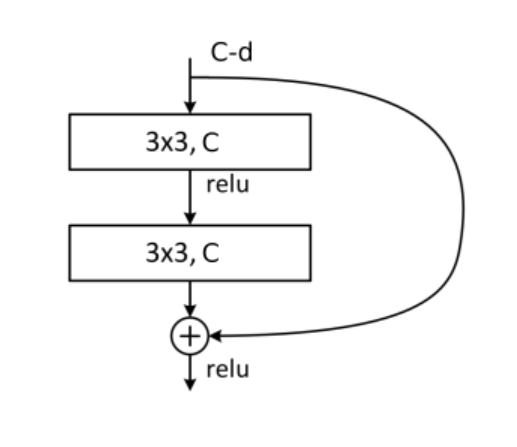
\includegraphics{residual_connection.png}
\caption{Residual connection}
\end{figure}

Note that we use `SAME' padding, no bias, and batch normalization after
each convolution. You do not need \texttt{nn.Sequential} here. The skip
connection is already implemented as \texttt{self.skip}. It can handle
different strides and increases in the number of channels.

    \begin{tcolorbox}[breakable, size=fbox, boxrule=1pt, pad at break*=1mm,colback=cellbackground, colframe=cellborder]
\prompt{In}{incolor}{7}{\hspace{4pt}}
\begin{Verbatim}[commandchars=\\\{\}]
\PY{k}{class} \PY{n+nc}{ResidualBlock}\PY{p}{(}\PY{n}{nn}\PY{o}{.}\PY{n}{Module}\PY{p}{)}\PY{p}{:}
    \PY{l+s+sd}{\PYZdq{}\PYZdq{}\PYZdq{}}
\PY{l+s+sd}{    The residual block used by ResNet.}
\PY{l+s+sd}{    }
\PY{l+s+sd}{    Args:}
\PY{l+s+sd}{        in\PYZus{}channels: The number of channels (feature maps) of the incoming embedding}
\PY{l+s+sd}{        out\PYZus{}channels: The number of channels after the first convolution}
\PY{l+s+sd}{        stride: Stride size of the first convolution, used for downsampling}
\PY{l+s+sd}{    \PYZdq{}\PYZdq{}\PYZdq{}}
    
    \PY{k}{def} \PY{n+nf}{\PYZus{}\PYZus{}init\PYZus{}\PYZus{}}\PY{p}{(}\PY{n+nb+bp}{self}\PY{p}{,} \PY{n}{in\PYZus{}channels}\PY{p}{,} \PY{n}{out\PYZus{}channels}\PY{p}{,} \PY{n}{stride}\PY{o}{=}\PY{l+m+mi}{1}\PY{p}{)}\PY{p}{:}
        \PY{n+nb}{super}\PY{p}{(}\PY{p}{)}\PY{o}{.}\PY{n+nf+fm}{\PYZus{}\PYZus{}init\PYZus{}\PYZus{}}\PY{p}{(}\PY{p}{)}        
        \PY{k}{if} \PY{n}{stride} \PY{o}{\PYZgt{}} \PY{l+m+mi}{1} \PY{o+ow}{or} \PY{n}{in\PYZus{}channels} \PY{o}{!=} \PY{n}{out\PYZus{}channels}\PY{p}{:}
            \PY{c+c1}{\PYZsh{} Add strides in the skip connection and zeros for the new channels.}
            \PY{n+nb+bp}{self}\PY{o}{.}\PY{n}{skip} \PY{o}{=} \PY{n}{Lambda}\PY{p}{(}\PY{k}{lambda} \PY{n}{x}\PY{p}{:} \PY{n}{F}\PY{o}{.}\PY{n}{pad}\PY{p}{(}\PY{n}{x}\PY{p}{[}\PY{p}{:}\PY{p}{,} \PY{p}{:}\PY{p}{,} \PY{p}{:}\PY{p}{:}\PY{n}{stride}\PY{p}{,} \PY{p}{:}\PY{p}{:}\PY{n}{stride}\PY{p}{]}\PY{p}{,}
                                               \PY{p}{(}\PY{l+m+mi}{0}\PY{p}{,} \PY{l+m+mi}{0}\PY{p}{,} \PY{l+m+mi}{0}\PY{p}{,} \PY{l+m+mi}{0}\PY{p}{,} \PY{l+m+mi}{0}\PY{p}{,} \PY{n}{out\PYZus{}channels} \PY{o}{\PYZhy{}} \PY{n}{in\PYZus{}channels}\PY{p}{)}\PY{p}{,}
                                               \PY{n}{mode}\PY{o}{=}\PY{l+s+s2}{\PYZdq{}}\PY{l+s+s2}{constant}\PY{l+s+s2}{\PYZdq{}}\PY{p}{,} \PY{n}{value}\PY{o}{=}\PY{l+m+mi}{0}\PY{p}{)}\PY{p}{)}
        \PY{k}{else}\PY{p}{:}
            \PY{n+nb+bp}{self}\PY{o}{.}\PY{n}{skip} \PY{o}{=} \PY{n}{nn}\PY{o}{.}\PY{n}{Sequential}\PY{p}{(}\PY{p}{)}
            
        \PY{c+c1}{\PYZsh{} TODO: Initialize the required layers}
        \PY{n+nb+bp}{self}\PY{o}{.}\PY{n}{left} \PY{o}{=} \PY{n}{nn}\PY{o}{.}\PY{n}{Sequential}\PY{p}{(}
            \PY{n}{nn}\PY{o}{.}\PY{n}{Conv2d}\PY{p}{(}\PY{n}{in\PYZus{}channels}\PY{p}{,} \PY{n}{out\PYZus{}channels}\PY{p}{,} \PY{n}{kernel\PYZus{}size}\PY{o}{=}\PY{l+m+mi}{3}\PY{p}{,} \PY{n}{stride}\PY{o}{=}\PY{n}{stride}\PY{p}{,} \PY{n}{padding}\PY{o}{=}\PY{l+m+mi}{1}\PY{p}{,} \PY{n}{bias}\PY{o}{=}\PY{k+kc}{False}\PY{p}{)}\PY{p}{,}
            \PY{n}{nn}\PY{o}{.}\PY{n}{BatchNorm2d}\PY{p}{(}\PY{n}{out\PYZus{}channels}\PY{p}{)}\PY{p}{,}
            \PY{n}{nn}\PY{o}{.}\PY{n}{ReLU}\PY{p}{(}\PY{n}{inplace}\PY{o}{=}\PY{k+kc}{True}\PY{p}{)}\PY{p}{,}
            \PY{n}{nn}\PY{o}{.}\PY{n}{Conv2d}\PY{p}{(}\PY{n}{out\PYZus{}channels}\PY{p}{,} \PY{n}{out\PYZus{}channels}\PY{p}{,} \PY{n}{kernel\PYZus{}size}\PY{o}{=}\PY{l+m+mi}{3}\PY{p}{,} \PY{n}{stride}\PY{o}{=}\PY{l+m+mi}{1}\PY{p}{,} \PY{n}{padding}\PY{o}{=}\PY{l+m+mi}{1}\PY{p}{,} \PY{n}{bias}\PY{o}{=}\PY{k+kc}{False}\PY{p}{)}\PY{p}{,}
            \PY{n}{nn}\PY{o}{.}\PY{n}{BatchNorm2d}\PY{p}{(}\PY{n}{out\PYZus{}channels}\PY{p}{)}
        \PY{p}{)}
        
        
        
    \PY{k}{def} \PY{n+nf}{forward}\PY{p}{(}\PY{n+nb+bp}{self}\PY{p}{,} \PY{n+nb}{input}\PY{p}{)}\PY{p}{:}
        \PY{c+c1}{\PYZsh{} TODO: Execute the required layers and functions}
        \PY{n}{out} \PY{o}{=} \PY{n+nb+bp}{self}\PY{o}{.}\PY{n}{left}\PY{p}{(}\PY{n+nb}{input}\PY{p}{)}
        \PY{n}{out} \PY{o}{+}\PY{o}{=} \PY{n+nb}{input}
        \PY{n}{out} \PY{o}{=} \PY{n}{F}\PY{o}{.}\PY{n}{relu}\PY{p}{(}\PY{n}{out}\PY{p}{)}
        \PY{k}{return} \PY{n}{out}
\end{Verbatim}
\end{tcolorbox}

    Next we implement a stack of residual blocks for convenience. The first
layer in the block is the one changing the number of channels and
downsampling. You can use \texttt{nn.ModuleList} to use a list of child
modules.

    \begin{tcolorbox}[breakable, size=fbox, boxrule=1pt, pad at break*=1mm,colback=cellbackground, colframe=cellborder]
\prompt{In}{incolor}{8}{\hspace{4pt}}
\begin{Verbatim}[commandchars=\\\{\}]
\PY{k}{class} \PY{n+nc}{ResidualStack}\PY{p}{(}\PY{n}{nn}\PY{o}{.}\PY{n}{Module}\PY{p}{)}\PY{p}{:}
    \PY{l+s+sd}{\PYZdq{}\PYZdq{}\PYZdq{}}
\PY{l+s+sd}{    A stack of residual blocks.}
\PY{l+s+sd}{    }
\PY{l+s+sd}{    Args:}
\PY{l+s+sd}{        in\PYZus{}channels: The number of channels (feature maps) of the incoming embedding}
\PY{l+s+sd}{        out\PYZus{}channels: The number of channels after the first layer}
\PY{l+s+sd}{        stride: Stride size of the first layer, used for downsampling}
\PY{l+s+sd}{        num\PYZus{}blocks: Number of residual blocks}
\PY{l+s+sd}{    \PYZdq{}\PYZdq{}\PYZdq{}}
    
    \PY{k}{def} \PY{n+nf}{\PYZus{}\PYZus{}init\PYZus{}\PYZus{}}\PY{p}{(}\PY{n+nb+bp}{self}\PY{p}{,} \PY{n}{in\PYZus{}channels}\PY{p}{,} \PY{n}{out\PYZus{}channels}\PY{p}{,} \PY{n}{stride}\PY{p}{,} \PY{n}{num\PYZus{}blocks}\PY{p}{)}\PY{p}{:}
        \PY{n+nb}{super}\PY{p}{(}\PY{p}{)}\PY{o}{.}\PY{n+nf+fm}{\PYZus{}\PYZus{}init\PYZus{}\PYZus{}}\PY{p}{(}\PY{p}{)}
        
        \PY{c+c1}{\PYZsh{} TODO: Initialize the required layers (blocks)}
        \PY{n+nb+bp}{self}\PY{o}{.}\PY{n}{\PYZus{}num\PYZus{}blocks} \PY{o}{=} \PY{n}{num\PYZus{}blocks}
        \PY{n+nb+bp}{self}\PY{o}{.}\PY{n}{\PYZus{}layers} \PY{o}{=} \PY{n}{nn}\PY{o}{.}\PY{n}{ModuleList}\PY{p}{(}\PY{p}{[}\PY{n}{ResidualBlock}\PY{p}{(}\PY{n}{out\PYZus{}channels}\PY{p}{,} \PY{n}{out\PYZus{}channels}\PY{p}{,} \PY{n}{stride}\PY{p}{)} \PY{k}{for} \PY{n}{\PYZus{}} \PY{o+ow}{in} \PY{n+nb}{range}\PY{p}{(}\PY{n+nb+bp}{self}\PY{o}{.}\PY{n}{\PYZus{}num\PYZus{}blocks} \PY{o}{\PYZhy{}} \PY{l+m+mi}{1}\PY{p}{)}\PY{p}{]}\PY{p}{)}
        
    \PY{k}{def} \PY{n+nf}{forward}\PY{p}{(}\PY{n+nb+bp}{self}\PY{p}{,} \PY{n+nb}{input}\PY{p}{)}\PY{p}{:}
        \PY{c+c1}{\PYZsh{} TODO: Execute the layers (blocks)}
        \PY{n+nb}{input} \PY{o}{=} \PY{n}{ResidualBlock}\PY{p}{(}\PY{n}{in\PYZus{}channels}\PY{p}{,} \PY{n}{out\PYZus{}channels}\PY{p}{,} \PY{n}{stride}\PY{o}{=}\PY{n}{stride}\PY{p}{)}
        \PY{k}{for} \PY{n}{i} \PY{o+ow}{in} \PY{n+nb}{range}\PY{p}{(}\PY{n+nb+bp}{self}\PY{o}{.}\PY{n}{\PYZus{}num\PYZus{}blocks} \PY{o}{\PYZhy{}} \PY{l+m+mi}{1}\PY{p}{)}\PY{p}{:}
            \PY{n+nb}{input} \PY{o}{=} \PY{n+nb+bp}{self}\PY{o}{.}\PY{n}{\PYZus{}layers}\PY{p}{[}\PY{n}{i}\PY{p}{]}\PY{p}{(}\PY{n+nb}{input}\PY{p}{)}
        \PY{k}{return} \PY{n}{F}\PY{o}{.}\PY{n}{relu}\PY{p}{(}\PY{n}{x}\PY{p}{)}
\end{Verbatim}
\end{tcolorbox}

    Now we are finally ready to implement the full model! To do this, use
the \texttt{nn.Sequential} API and carefully read the following
paragraph from the paper (Fig. 3 is not important):

\begin{figure}
\centering
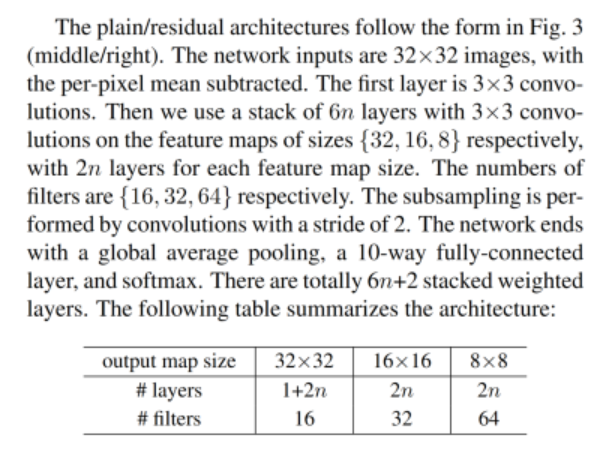
\includegraphics{resnet_cifar10_description.png}
\caption{ResNet CIFAR10 description}
\end{figure}

Note that a convolution layer is always convolution + batch norm +
activation (ReLU), that each ResidualBlock contains 2 layers, and that
you might have to \texttt{squeeze} the embedding before the dense
(fully-connected) layer.

    \begin{tcolorbox}[breakable, size=fbox, boxrule=1pt, pad at break*=1mm,colback=cellbackground, colframe=cellborder]
\prompt{In}{incolor}{9}{\hspace{4pt}}
\begin{Verbatim}[commandchars=\\\{\}]
\PY{n}{n} \PY{o}{=} \PY{l+m+mi}{5}
\PY{n}{num\PYZus{}classes} \PY{o}{=} \PY{l+m+mi}{10}

\PY{c+c1}{\PYZsh{} TODO: Implement ResNet via nn.Sequential}
\PY{n}{num\PYZus{}blocks} \PY{o}{=} \PY{n}{n}
\PY{k}{class} \PY{n+nc}{ResNet}\PY{p}{(}\PY{n}{nn}\PY{o}{.}\PY{n}{Module}\PY{p}{)}\PY{p}{:}
    \PY{k}{def} \PY{n+nf}{\PYZus{}\PYZus{}init\PYZus{}\PYZus{}}\PY{p}{(}\PY{n+nb+bp}{self}\PY{p}{,} \PY{n}{ResidualBlock}\PY{p}{,} \PY{n}{num\PYZus{}classes}\PY{o}{=}\PY{l+m+mi}{10}\PY{p}{)}\PY{p}{:}
        \PY{n+nb}{super}\PY{p}{(}\PY{n}{ResNet}\PY{p}{,} \PY{n+nb+bp}{self}\PY{p}{)}\PY{o}{.}\PY{n+nf+fm}{\PYZus{}\PYZus{}init\PYZus{}\PYZus{}}\PY{p}{(}\PY{p}{)}
        \PY{n+nb+bp}{self}\PY{o}{.}\PY{n}{inchannel} \PY{o}{=} \PY{l+m+mi}{64}
        \PY{n+nb+bp}{self}\PY{o}{.}\PY{n}{conv1} \PY{o}{=} \PY{n}{nn}\PY{o}{.}\PY{n}{Sequential}\PY{p}{(}
            \PY{n}{nn}\PY{o}{.}\PY{n}{Conv2d}\PY{p}{(}\PY{l+m+mi}{3}\PY{p}{,} \PY{l+m+mi}{64}\PY{p}{,} \PY{n}{kernel\PYZus{}size}\PY{o}{=}\PY{l+m+mi}{3}\PY{p}{,} \PY{n}{stride}\PY{o}{=}\PY{l+m+mi}{1}\PY{p}{,} \PY{n}{padding}\PY{o}{=}\PY{l+m+mi}{1}\PY{p}{,} \PY{n}{bias}\PY{o}{=}\PY{k+kc}{False}\PY{p}{)}\PY{p}{,}
            \PY{n}{nn}\PY{o}{.}\PY{n}{BatchNorm2d}\PY{p}{(}\PY{l+m+mi}{64}\PY{p}{)}\PY{p}{,}
            \PY{n}{nn}\PY{o}{.}\PY{n}{ReLU}\PY{p}{(}\PY{p}{)}\PY{p}{,}
        \PY{p}{)}
        \PY{n+nb+bp}{self}\PY{o}{.}\PY{n}{layer1} \PY{o}{=} \PY{n+nb+bp}{self}\PY{o}{.}\PY{n}{make\PYZus{}layer}\PY{p}{(}\PY{n}{ResidualBlock}\PY{p}{,} \PY{l+m+mi}{64}\PY{p}{,}  \PY{l+m+mi}{2}\PY{p}{,} \PY{n}{stride}\PY{o}{=}\PY{l+m+mi}{1}\PY{p}{)}
        \PY{n+nb+bp}{self}\PY{o}{.}\PY{n}{layer2} \PY{o}{=} \PY{n+nb+bp}{self}\PY{o}{.}\PY{n}{make\PYZus{}layer}\PY{p}{(}\PY{n}{ResidualBlock}\PY{p}{,} \PY{l+m+mi}{128}\PY{p}{,} \PY{l+m+mi}{2}\PY{p}{,} \PY{n}{stride}\PY{o}{=}\PY{l+m+mi}{2}\PY{p}{)}
        \PY{n+nb+bp}{self}\PY{o}{.}\PY{n}{layer3} \PY{o}{=} \PY{n+nb+bp}{self}\PY{o}{.}\PY{n}{make\PYZus{}layer}\PY{p}{(}\PY{n}{ResidualBlock}\PY{p}{,} \PY{l+m+mi}{256}\PY{p}{,} \PY{l+m+mi}{2}\PY{p}{,} \PY{n}{stride}\PY{o}{=}\PY{l+m+mi}{2}\PY{p}{)}
        \PY{n+nb+bp}{self}\PY{o}{.}\PY{n}{layer4} \PY{o}{=} \PY{n+nb+bp}{self}\PY{o}{.}\PY{n}{make\PYZus{}layer}\PY{p}{(}\PY{n}{ResidualBlock}\PY{p}{,} \PY{l+m+mi}{512}\PY{p}{,} \PY{l+m+mi}{2}\PY{p}{,} \PY{n}{stride}\PY{o}{=}\PY{l+m+mi}{2}\PY{p}{)}
        \PY{n+nb+bp}{self}\PY{o}{.}\PY{n}{fc} \PY{o}{=} \PY{n}{nn}\PY{o}{.}\PY{n}{Linear}\PY{p}{(}\PY{l+m+mi}{512}\PY{p}{,} \PY{n}{num\PYZus{}classes}\PY{p}{)}

    \PY{k}{def} \PY{n+nf}{make\PYZus{}layer}\PY{p}{(}\PY{n+nb+bp}{self}\PY{p}{,} \PY{n}{block}\PY{p}{,} \PY{n}{channels}\PY{p}{,} \PY{n}{num\PYZus{}blocks}\PY{p}{,} \PY{n}{stride}\PY{p}{)}\PY{p}{:}
        \PY{n}{strides} \PY{o}{=} \PY{p}{[}\PY{n}{stride}\PY{p}{]} \PY{o}{+} \PY{p}{[}\PY{l+m+mi}{1}\PY{p}{]} \PY{o}{*} \PY{p}{(}\PY{n}{num\PYZus{}blocks} \PY{o}{\PYZhy{}} \PY{l+m+mi}{1}\PY{p}{)}   \PY{c+c1}{\PYZsh{}strides=[1,1]}
        \PY{n}{layers} \PY{o}{=} \PY{p}{[}\PY{p}{]}
        \PY{k}{for} \PY{n}{stride} \PY{o+ow}{in} \PY{n}{strides}\PY{p}{:}
            \PY{n}{layers}\PY{o}{.}\PY{n}{append}\PY{p}{(}\PY{n}{block}\PY{p}{(}\PY{n+nb+bp}{self}\PY{o}{.}\PY{n}{inchannel}\PY{p}{,} \PY{n}{channels}\PY{p}{,} \PY{n}{stride}\PY{p}{)}\PY{p}{)}
            \PY{n+nb+bp}{self}\PY{o}{.}\PY{n}{inchannel} \PY{o}{=} \PY{n}{channels}
        \PY{k}{return} \PY{n}{nn}\PY{o}{.}\PY{n}{Sequential}\PY{p}{(}\PY{o}{*}\PY{n}{layers}\PY{p}{)}

    \PY{k}{def} \PY{n+nf}{forward}\PY{p}{(}\PY{n+nb+bp}{self}\PY{p}{,} \PY{n}{x}\PY{p}{)}\PY{p}{:}
        \PY{n}{out} \PY{o}{=} \PY{n+nb+bp}{self}\PY{o}{.}\PY{n}{conv1}\PY{p}{(}\PY{n}{x}\PY{p}{)}
        \PY{n}{out} \PY{o}{=} \PY{n+nb+bp}{self}\PY{o}{.}\PY{n}{layer1}\PY{p}{(}\PY{n}{out}\PY{p}{)}
        \PY{n}{out} \PY{o}{=} \PY{n+nb+bp}{self}\PY{o}{.}\PY{n}{layer2}\PY{p}{(}\PY{n}{out}\PY{p}{)}
        \PY{n}{out} \PY{o}{=} \PY{n+nb+bp}{self}\PY{o}{.}\PY{n}{layer3}\PY{p}{(}\PY{n}{out}\PY{p}{)}
        \PY{n}{out} \PY{o}{=} \PY{n+nb+bp}{self}\PY{o}{.}\PY{n}{layer4}\PY{p}{(}\PY{n}{out}\PY{p}{)}
        \PY{n}{out} \PY{o}{=} \PY{n}{F}\PY{o}{.}\PY{n}{avg\PYZus{}pool2d}\PY{p}{(}\PY{n}{out}\PY{p}{,} \PY{l+m+mi}{4}\PY{p}{)}
        \PY{n}{out} \PY{o}{=} \PY{n}{out}\PY{o}{.}\PY{n}{view}\PY{p}{(}\PY{n}{out}\PY{o}{.}\PY{n}{size}\PY{p}{(}\PY{l+m+mi}{0}\PY{p}{)}\PY{p}{,} \PY{o}{\PYZhy{}}\PY{l+m+mi}{1}\PY{p}{)}
        \PY{n}{out} \PY{o}{=} \PY{n+nb+bp}{self}\PY{o}{.}\PY{n}{fc}\PY{p}{(}\PY{n}{out}\PY{p}{)}
        \PY{k}{return} \PY{n}{out}

\PY{n}{resnet} \PY{o}{=} \PY{n}{ResNet}\PY{p}{(}\PY{n}{ResidualBlock}\PY{p}{)}
\end{Verbatim}
\end{tcolorbox}

    Next we need to initialize the weights of our model.

    \begin{tcolorbox}[breakable, size=fbox, boxrule=1pt, pad at break*=1mm,colback=cellbackground, colframe=cellborder]
\prompt{In}{incolor}{10}{\hspace{4pt}}
\begin{Verbatim}[commandchars=\\\{\}]
\PY{k}{def} \PY{n+nf}{initialize\PYZus{}weight}\PY{p}{(}\PY{n}{module}\PY{p}{)}\PY{p}{:}
    \PY{k}{if} \PY{n+nb}{isinstance}\PY{p}{(}\PY{n}{module}\PY{p}{,} \PY{p}{(}\PY{n}{nn}\PY{o}{.}\PY{n}{Linear}\PY{p}{,} \PY{n}{nn}\PY{o}{.}\PY{n}{Conv2d}\PY{p}{)}\PY{p}{)}\PY{p}{:}
        \PY{n}{nn}\PY{o}{.}\PY{n}{init}\PY{o}{.}\PY{n}{kaiming\PYZus{}normal\PYZus{}}\PY{p}{(}\PY{n}{module}\PY{o}{.}\PY{n}{weight}\PY{p}{,} \PY{n}{nonlinearity}\PY{o}{=}\PY{l+s+s1}{\PYZsq{}}\PY{l+s+s1}{relu}\PY{l+s+s1}{\PYZsq{}}\PY{p}{)}
    \PY{k}{elif} \PY{n+nb}{isinstance}\PY{p}{(}\PY{n}{module}\PY{p}{,} \PY{n}{nn}\PY{o}{.}\PY{n}{BatchNorm2d}\PY{p}{)}\PY{p}{:}
        \PY{n}{nn}\PY{o}{.}\PY{n}{init}\PY{o}{.}\PY{n}{constant\PYZus{}}\PY{p}{(}\PY{n}{module}\PY{o}{.}\PY{n}{weight}\PY{p}{,} \PY{l+m+mi}{1}\PY{p}{)}
        \PY{n}{nn}\PY{o}{.}\PY{n}{init}\PY{o}{.}\PY{n}{constant\PYZus{}}\PY{p}{(}\PY{n}{module}\PY{o}{.}\PY{n}{bias}\PY{p}{,} \PY{l+m+mi}{0}\PY{p}{)}
        
\PY{n}{resnet}\PY{o}{.}\PY{n}{apply}\PY{p}{(}\PY{n}{initialize\PYZus{}weight}\PY{p}{)}\PY{p}{;}
\end{Verbatim}
\end{tcolorbox}

    \hypertarget{training}{%
\section{4. Training}\label{training}}

So now we have a shiny new model, but that doesn't really help when we
can't train it. So that's what we do next.

First we need to load the data. Note that we split the official training
data into train and validation sets, because you must not look at the
test set until you are completely done developing your model and report
the final results. Some people don't do this properly, but you should
not copy other people's bad habits.

    \begin{tcolorbox}[breakable, size=fbox, boxrule=1pt, pad at break*=1mm,colback=cellbackground, colframe=cellborder]
\prompt{In}{incolor}{11}{\hspace{4pt}}
\begin{Verbatim}[commandchars=\\\{\}]
\PY{k}{class} \PY{n+nc}{CIFAR10Subset}\PY{p}{(}\PY{n}{torchvision}\PY{o}{.}\PY{n}{datasets}\PY{o}{.}\PY{n}{CIFAR10}\PY{p}{)}\PY{p}{:}
    \PY{l+s+sd}{\PYZdq{}\PYZdq{}\PYZdq{}}
\PY{l+s+sd}{    Get a subset of the CIFAR10 dataset, according to the passed indices.}
\PY{l+s+sd}{    \PYZdq{}\PYZdq{}\PYZdq{}}
    \PY{k}{def} \PY{n+nf}{\PYZus{}\PYZus{}init\PYZus{}\PYZus{}}\PY{p}{(}\PY{n+nb+bp}{self}\PY{p}{,} \PY{o}{*}\PY{n}{args}\PY{p}{,} \PY{n}{idx}\PY{o}{=}\PY{k+kc}{None}\PY{p}{,} \PY{o}{*}\PY{o}{*}\PY{n}{kwargs}\PY{p}{)}\PY{p}{:}
        \PY{n+nb}{super}\PY{p}{(}\PY{p}{)}\PY{o}{.}\PY{n+nf+fm}{\PYZus{}\PYZus{}init\PYZus{}\PYZus{}}\PY{p}{(}\PY{o}{*}\PY{n}{args}\PY{p}{,} \PY{o}{*}\PY{o}{*}\PY{n}{kwargs}\PY{p}{)}
        
        \PY{k}{if} \PY{n}{idx} \PY{o+ow}{is} \PY{k+kc}{None}\PY{p}{:}
            \PY{k}{return}
        
        \PY{n+nb+bp}{self}\PY{o}{.}\PY{n}{data} \PY{o}{=} \PY{n+nb+bp}{self}\PY{o}{.}\PY{n}{data}\PY{p}{[}\PY{n}{idx}\PY{p}{]}
        \PY{n}{targets\PYZus{}np} \PY{o}{=} \PY{n}{np}\PY{o}{.}\PY{n}{array}\PY{p}{(}\PY{n+nb+bp}{self}\PY{o}{.}\PY{n}{targets}\PY{p}{)}
        \PY{n+nb+bp}{self}\PY{o}{.}\PY{n}{targets} \PY{o}{=} \PY{n}{targets\PYZus{}np}\PY{p}{[}\PY{n}{idx}\PY{p}{]}\PY{o}{.}\PY{n}{tolist}\PY{p}{(}\PY{p}{)}
\end{Verbatim}
\end{tcolorbox}

    We next define transformations that change the images into PyTorch
tensors, standardize the values according to the precomputed mean and
standard deviation, and provide data augmentation for the training set.

    \begin{tcolorbox}[breakable, size=fbox, boxrule=1pt, pad at break*=1mm,colback=cellbackground, colframe=cellborder]
\prompt{In}{incolor}{12}{\hspace{4pt}}
\begin{Verbatim}[commandchars=\\\{\}]
\PY{n}{normalize} \PY{o}{=} \PY{n}{transforms}\PY{o}{.}\PY{n}{Normalize}\PY{p}{(}\PY{n}{mean}\PY{o}{=}\PY{p}{[}\PY{l+m+mf}{0.485}\PY{p}{,} \PY{l+m+mf}{0.456}\PY{p}{,} \PY{l+m+mf}{0.406}\PY{p}{]}\PY{p}{,}
                                 \PY{n}{std}\PY{o}{=}\PY{p}{[}\PY{l+m+mf}{0.229}\PY{p}{,} \PY{l+m+mf}{0.224}\PY{p}{,} \PY{l+m+mf}{0.225}\PY{p}{]}\PY{p}{)}
\PY{n}{transform\PYZus{}train} \PY{o}{=} \PY{n}{transforms}\PY{o}{.}\PY{n}{Compose}\PY{p}{(}\PY{p}{[}
    \PY{n}{transforms}\PY{o}{.}\PY{n}{RandomHorizontalFlip}\PY{p}{(}\PY{p}{)}\PY{p}{,}
    \PY{n}{transforms}\PY{o}{.}\PY{n}{RandomCrop}\PY{p}{(}\PY{l+m+mi}{32}\PY{p}{,} \PY{l+m+mi}{4}\PY{p}{)}\PY{p}{,}
    \PY{n}{transforms}\PY{o}{.}\PY{n}{ToTensor}\PY{p}{(}\PY{p}{)}\PY{p}{,}
    \PY{n}{normalize}\PY{p}{,}
\PY{p}{]}\PY{p}{)}
\PY{n}{transform\PYZus{}eval} \PY{o}{=} \PY{n}{transforms}\PY{o}{.}\PY{n}{Compose}\PY{p}{(}\PY{p}{[}
    \PY{n}{transforms}\PY{o}{.}\PY{n}{ToTensor}\PY{p}{(}\PY{p}{)}\PY{p}{,}
    \PY{n}{normalize}
\PY{p}{]}\PY{p}{)}
\end{Verbatim}
\end{tcolorbox}

    \begin{tcolorbox}[breakable, size=fbox, boxrule=1pt, pad at break*=1mm,colback=cellbackground, colframe=cellborder]
\prompt{In}{incolor}{13}{\hspace{4pt}}
\begin{Verbatim}[commandchars=\\\{\}]
\PY{n}{ntrain} \PY{o}{=} \PY{l+m+mi}{45\PYZus{}000}
\PY{n}{train\PYZus{}set} \PY{o}{=} \PY{n}{CIFAR10Subset}\PY{p}{(}\PY{n}{root}\PY{o}{=}\PY{l+s+s1}{\PYZsq{}}\PY{l+s+s1}{./data}\PY{l+s+s1}{\PYZsq{}}\PY{p}{,} \PY{n}{train}\PY{o}{=}\PY{k+kc}{True}\PY{p}{,} \PY{n}{idx}\PY{o}{=}\PY{n+nb}{range}\PY{p}{(}\PY{n}{ntrain}\PY{p}{)}\PY{p}{,}
                          \PY{n}{download}\PY{o}{=}\PY{k+kc}{False}\PY{p}{,} \PY{n}{transform}\PY{o}{=}\PY{n}{transform\PYZus{}train}\PY{p}{)}
\PY{n}{val\PYZus{}set} \PY{o}{=} \PY{n}{CIFAR10Subset}\PY{p}{(}\PY{n}{root}\PY{o}{=}\PY{l+s+s1}{\PYZsq{}}\PY{l+s+s1}{./data}\PY{l+s+s1}{\PYZsq{}}\PY{p}{,} \PY{n}{train}\PY{o}{=}\PY{k+kc}{True}\PY{p}{,} \PY{n}{idx}\PY{o}{=}\PY{n+nb}{range}\PY{p}{(}\PY{n}{ntrain}\PY{p}{,} \PY{l+m+mi}{50\PYZus{}000}\PY{p}{)}\PY{p}{,}
                        \PY{n}{download}\PY{o}{=}\PY{k+kc}{False}\PY{p}{,} \PY{n}{transform}\PY{o}{=}\PY{n}{transform\PYZus{}eval}\PY{p}{)}
\PY{n}{test\PYZus{}set} \PY{o}{=} \PY{n}{torchvision}\PY{o}{.}\PY{n}{datasets}\PY{o}{.}\PY{n}{CIFAR10}\PY{p}{(}\PY{n}{root}\PY{o}{=}\PY{l+s+s1}{\PYZsq{}}\PY{l+s+s1}{./data}\PY{l+s+s1}{\PYZsq{}}\PY{p}{,} \PY{n}{train}\PY{o}{=}\PY{k+kc}{False}\PY{p}{,}
                                        \PY{n}{download}\PY{o}{=}\PY{k+kc}{False}\PY{p}{,} \PY{n}{transform}\PY{o}{=}\PY{n}{transform\PYZus{}eval}\PY{p}{)}
\end{Verbatim}
\end{tcolorbox}

    \begin{tcolorbox}[breakable, size=fbox, boxrule=1pt, pad at break*=1mm,colback=cellbackground, colframe=cellborder]
\prompt{In}{incolor}{14}{\hspace{4pt}}
\begin{Verbatim}[commandchars=\\\{\}]
\PY{n}{dataloaders} \PY{o}{=} \PY{p}{\PYZob{}}\PY{p}{\PYZcb{}}
\PY{n}{dataloaders}\PY{p}{[}\PY{l+s+s1}{\PYZsq{}}\PY{l+s+s1}{train}\PY{l+s+s1}{\PYZsq{}}\PY{p}{]} \PY{o}{=} \PY{n}{torch}\PY{o}{.}\PY{n}{utils}\PY{o}{.}\PY{n}{data}\PY{o}{.}\PY{n}{DataLoader}\PY{p}{(}\PY{n}{train\PYZus{}set}\PY{p}{,} \PY{n}{batch\PYZus{}size}\PY{o}{=}\PY{l+m+mi}{128}\PY{p}{,}
                                                   \PY{n}{shuffle}\PY{o}{=}\PY{k+kc}{True}\PY{p}{,} \PY{n}{num\PYZus{}workers}\PY{o}{=}\PY{l+m+mi}{2}\PY{p}{,}
                                                   \PY{n}{pin\PYZus{}memory}\PY{o}{=}\PY{k+kc}{True}\PY{p}{)}
\PY{n}{dataloaders}\PY{p}{[}\PY{l+s+s1}{\PYZsq{}}\PY{l+s+s1}{val}\PY{l+s+s1}{\PYZsq{}}\PY{p}{]} \PY{o}{=} \PY{n}{torch}\PY{o}{.}\PY{n}{utils}\PY{o}{.}\PY{n}{data}\PY{o}{.}\PY{n}{DataLoader}\PY{p}{(}\PY{n}{val\PYZus{}set}\PY{p}{,} \PY{n}{batch\PYZus{}size}\PY{o}{=}\PY{l+m+mi}{128}\PY{p}{,}
                                                 \PY{n}{shuffle}\PY{o}{=}\PY{k+kc}{False}\PY{p}{,} \PY{n}{num\PYZus{}workers}\PY{o}{=}\PY{l+m+mi}{2}\PY{p}{,}
                                                 \PY{n}{pin\PYZus{}memory}\PY{o}{=}\PY{k+kc}{True}\PY{p}{)}
\PY{n}{dataloaders}\PY{p}{[}\PY{l+s+s1}{\PYZsq{}}\PY{l+s+s1}{test}\PY{l+s+s1}{\PYZsq{}}\PY{p}{]} \PY{o}{=} \PY{n}{torch}\PY{o}{.}\PY{n}{utils}\PY{o}{.}\PY{n}{data}\PY{o}{.}\PY{n}{DataLoader}\PY{p}{(}\PY{n}{test\PYZus{}set}\PY{p}{,} \PY{n}{batch\PYZus{}size}\PY{o}{=}\PY{l+m+mi}{128}\PY{p}{,}
                                                  \PY{n}{shuffle}\PY{o}{=}\PY{k+kc}{False}\PY{p}{,} \PY{n}{num\PYZus{}workers}\PY{o}{=}\PY{l+m+mi}{2}\PY{p}{,}
                                                  \PY{n}{pin\PYZus{}memory}\PY{o}{=}\PY{k+kc}{True}\PY{p}{)}
\end{Verbatim}
\end{tcolorbox}

    Next we push the model to our GPU (if there is one).

    \begin{tcolorbox}[breakable, size=fbox, boxrule=1pt, pad at break*=1mm,colback=cellbackground, colframe=cellborder]
\prompt{In}{incolor}{15}{\hspace{4pt}}
\begin{Verbatim}[commandchars=\\\{\}]
\PY{n}{device} \PY{o}{=} \PY{n}{torch}\PY{o}{.}\PY{n}{device}\PY{p}{(}\PY{l+s+s1}{\PYZsq{}}\PY{l+s+s1}{cuda}\PY{l+s+s1}{\PYZsq{}}\PY{p}{)} \PY{k}{if} \PY{n}{torch}\PY{o}{.}\PY{n}{cuda}\PY{o}{.}\PY{n}{is\PYZus{}available}\PY{p}{(}\PY{p}{)} \PY{k}{else} \PY{n}{torch}\PY{o}{.}\PY{n}{device}\PY{p}{(}\PY{l+s+s1}{\PYZsq{}}\PY{l+s+s1}{cpu}\PY{l+s+s1}{\PYZsq{}}\PY{p}{)}
\PY{n}{resnet}\PY{o}{.}\PY{n}{to}\PY{p}{(}\PY{n}{device}\PY{p}{)}\PY{p}{;}
\end{Verbatim}
\end{tcolorbox}

    Next we define a helper method that does one epoch of training or
evaluation. We have only defined training here, so you need to implement
the necessary changes for evaluation!

    \begin{tcolorbox}[breakable, size=fbox, boxrule=1pt, pad at break*=1mm,colback=cellbackground, colframe=cellborder]
\prompt{In}{incolor}{16}{\hspace{4pt}}
\begin{Verbatim}[commandchars=\\\{\}]
\PY{k}{def} \PY{n+nf}{run\PYZus{}epoch}\PY{p}{(}\PY{n}{model}\PY{p}{,} \PY{n}{optimizer}\PY{p}{,} \PY{n}{dataloader}\PY{p}{,} \PY{n}{train}\PY{p}{)}\PY{p}{:}
    \PY{l+s+sd}{\PYZdq{}\PYZdq{}\PYZdq{}}
\PY{l+s+sd}{    Run one epoch of training or evaluation.}
\PY{l+s+sd}{    }
\PY{l+s+sd}{    Args:}
\PY{l+s+sd}{        model: The model used for prediction}
\PY{l+s+sd}{        optimizer: Optimization algorithm for the model}
\PY{l+s+sd}{        dataloader: Dataloader providing the data to run our model on}
\PY{l+s+sd}{        train: Whether this epoch is used for training or evaluation}
\PY{l+s+sd}{        }
\PY{l+s+sd}{    Returns:}
\PY{l+s+sd}{        Loss and accuracy in this epoch.}
\PY{l+s+sd}{    \PYZdq{}\PYZdq{}\PYZdq{}}
    \PY{c+c1}{\PYZsh{} TODO: Change the necessary parts to work correctly during evaluation (train=False)}
    
    \PY{n}{device} \PY{o}{=} \PY{n+nb}{next}\PY{p}{(}\PY{n}{model}\PY{o}{.}\PY{n}{parameters}\PY{p}{(}\PY{p}{)}\PY{p}{)}\PY{o}{.}\PY{n}{device}
    
    \PY{c+c1}{\PYZsh{} Set model to training mode (for e.g. batch normalization, dropout)}
    \PY{n}{model}\PY{o}{.}\PY{n}{train}\PY{p}{(}\PY{p}{)}

    \PY{n}{epoch\PYZus{}loss} \PY{o}{=} \PY{l+m+mf}{0.0}
    \PY{n}{epoch\PYZus{}acc} \PY{o}{=} \PY{l+m+mf}{0.0}

    \PY{c+c1}{\PYZsh{} Iterate over data}
    \PY{k}{for} \PY{n}{xb}\PY{p}{,} \PY{n}{yb} \PY{o+ow}{in} \PY{n}{dataloader}\PY{p}{:}
        \PY{n}{xb}\PY{p}{,} \PY{n}{yb} \PY{o}{=} \PY{n}{xb}\PY{o}{.}\PY{n}{to}\PY{p}{(}\PY{n}{device}\PY{p}{)}\PY{p}{,} \PY{n}{yb}\PY{o}{.}\PY{n}{to}\PY{p}{(}\PY{n}{device}\PY{p}{)}

        \PY{c+c1}{\PYZsh{} zero the parameter gradients}
        \PY{n}{optimizer}\PY{o}{.}\PY{n}{zero\PYZus{}grad}\PY{p}{(}\PY{p}{)}

        \PY{c+c1}{\PYZsh{} forward}
        \PY{k}{with} \PY{n}{torch}\PY{o}{.}\PY{n}{set\PYZus{}grad\PYZus{}enabled}\PY{p}{(}\PY{k+kc}{True}\PY{p}{)}\PY{p}{:}
            \PY{n}{pred} \PY{o}{=} \PY{n}{model}\PY{p}{(}\PY{n}{xb}\PY{p}{)}
            \PY{n}{loss} \PY{o}{=} \PY{n}{F}\PY{o}{.}\PY{n}{cross\PYZus{}entropy}\PY{p}{(}\PY{n}{pred}\PY{p}{,} \PY{n}{yb}\PY{p}{)}
            \PY{n}{top1} \PY{o}{=} \PY{n}{torch}\PY{o}{.}\PY{n}{argmax}\PY{p}{(}\PY{n}{pred}\PY{p}{,} \PY{n}{dim}\PY{o}{=}\PY{l+m+mi}{1}\PY{p}{)}
            \PY{n}{ncorrect} \PY{o}{=} \PY{n}{torch}\PY{o}{.}\PY{n}{sum}\PY{p}{(}\PY{n}{top1} \PY{o}{==} \PY{n}{yb}\PY{p}{)}

            \PY{n}{loss}\PY{o}{.}\PY{n}{backward}\PY{p}{(}\PY{p}{)}
            \PY{n}{optimizer}\PY{o}{.}\PY{n}{step}\PY{p}{(}\PY{p}{)}

        \PY{c+c1}{\PYZsh{} statistics}
        \PY{n}{epoch\PYZus{}loss} \PY{o}{+}\PY{o}{=} \PY{n}{loss}\PY{o}{.}\PY{n}{item}\PY{p}{(}\PY{p}{)}
        \PY{n}{epoch\PYZus{}acc} \PY{o}{+}\PY{o}{=} \PY{n}{ncorrect}\PY{o}{.}\PY{n}{item}\PY{p}{(}\PY{p}{)}
    
    \PY{n}{epoch\PYZus{}loss} \PY{o}{/}\PY{o}{=} \PY{n+nb}{len}\PY{p}{(}\PY{n}{dataloader}\PY{o}{.}\PY{n}{dataset}\PY{p}{)}
    \PY{n}{epoch\PYZus{}acc} \PY{o}{/}\PY{o}{=} \PY{n+nb}{len}\PY{p}{(}\PY{n}{dataloader}\PY{o}{.}\PY{n}{dataset}\PY{p}{)}
    \PY{k}{return} \PY{n}{epoch\PYZus{}loss}\PY{p}{,} \PY{n}{epoch\PYZus{}acc}
\end{Verbatim}
\end{tcolorbox}

    Next we implement a method for fitting (training) our model. For many
models early stopping can save a lot of training time. Your task is to
add early stopping to the loop (based on validation accuracy). Early
stopping usually means exiting the training loop if the validation
accuracy hasn't improved for \texttt{patience} number of steps. Don't
forget to save the best model parameters according to validation
accuracy. You will need \texttt{copy.deepcopy} and the
\texttt{state\_dict} for this.

    \begin{tcolorbox}[breakable, size=fbox, boxrule=1pt, pad at break*=1mm,colback=cellbackground, colframe=cellborder]
\prompt{In}{incolor}{17}{\hspace{4pt}}
\begin{Verbatim}[commandchars=\\\{\}]
\PY{k}{def} \PY{n+nf}{fit}\PY{p}{(}\PY{n}{model}\PY{p}{,} \PY{n}{optimizer}\PY{p}{,} \PY{n}{lr\PYZus{}scheduler}\PY{p}{,} \PY{n}{dataloaders}\PY{p}{,} \PY{n}{max\PYZus{}epochs}\PY{p}{,} \PY{n}{patience}\PY{p}{)}\PY{p}{:}
    \PY{l+s+sd}{\PYZdq{}\PYZdq{}\PYZdq{}}
\PY{l+s+sd}{    Fit the given model on the dataset.}
\PY{l+s+sd}{    }
\PY{l+s+sd}{    Args:}
\PY{l+s+sd}{        model: The model used for prediction}
\PY{l+s+sd}{        optimizer: Optimization algorithm for the model}
\PY{l+s+sd}{        lr\PYZus{}scheduler: Learning rate scheduler that improves training}
\PY{l+s+sd}{                      in late epochs with learning rate decay}
\PY{l+s+sd}{        dataloaders: Dataloaders for training and validation}
\PY{l+s+sd}{        max\PYZus{}epochs: Maximum number of epochs for training}
\PY{l+s+sd}{        patience: Number of epochs to wait with early stopping the}
\PY{l+s+sd}{                  training if validation loss has decreased}
\PY{l+s+sd}{                  }
\PY{l+s+sd}{    Returns:}
\PY{l+s+sd}{        Loss and accuracy in this epoch.}
\PY{l+s+sd}{    \PYZdq{}\PYZdq{}\PYZdq{}}
    
    \PY{n}{best\PYZus{}acc} \PY{o}{=} \PY{l+m+mi}{0}
    \PY{n}{curr\PYZus{}patience} \PY{o}{=} \PY{l+m+mi}{0}
    
    \PY{k}{for} \PY{n}{epoch} \PY{o+ow}{in} \PY{n+nb}{range}\PY{p}{(}\PY{n}{max\PYZus{}epochs}\PY{p}{)}\PY{p}{:}
        \PY{n}{train\PYZus{}loss}\PY{p}{,} \PY{n}{train\PYZus{}acc} \PY{o}{=} \PY{n}{run\PYZus{}epoch}\PY{p}{(}\PY{n}{model}\PY{p}{,} \PY{n}{optimizer}\PY{p}{,} \PY{n}{dataloaders}\PY{p}{[}\PY{l+s+s1}{\PYZsq{}}\PY{l+s+s1}{train}\PY{l+s+s1}{\PYZsq{}}\PY{p}{]}\PY{p}{,} \PY{n}{train}\PY{o}{=}\PY{k+kc}{True}\PY{p}{)}
        \PY{n}{lr\PYZus{}scheduler}\PY{o}{.}\PY{n}{step}\PY{p}{(}\PY{p}{)}
        \PY{n+nb}{print}\PY{p}{(}\PY{n}{f}\PY{l+s+s2}{\PYZdq{}}\PY{l+s+s2}{Epoch }\PY{l+s+s2}{\PYZob{}}\PY{l+s+s2}{epoch + 1: \PYZgt{}3\PYZcb{}/}\PY{l+s+si}{\PYZob{}max\PYZus{}epochs\PYZcb{}}\PY{l+s+s2}{, train loss: }\PY{l+s+si}{\PYZob{}train\PYZus{}loss:.2e\PYZcb{}}\PY{l+s+s2}{, accuracy: }\PY{l+s+s2}{\PYZob{}}\PY{l+s+s2}{train\PYZus{}acc * 100:.2f\PYZcb{}}\PY{l+s+s2}{\PYZpc{}}\PY{l+s+s2}{\PYZdq{}}\PY{p}{)}
        
        \PY{n}{val\PYZus{}loss}\PY{p}{,} \PY{n}{val\PYZus{}acc} \PY{o}{=} \PY{n}{run\PYZus{}epoch}\PY{p}{(}\PY{n}{model}\PY{p}{,} \PY{k+kc}{None}\PY{p}{,} \PY{n}{dataloaders}\PY{p}{[}\PY{l+s+s1}{\PYZsq{}}\PY{l+s+s1}{val}\PY{l+s+s1}{\PYZsq{}}\PY{p}{]}\PY{p}{,} \PY{n}{train}\PY{o}{=}\PY{k+kc}{False}\PY{p}{)}
        \PY{n+nb}{print}\PY{p}{(}\PY{n}{f}\PY{l+s+s2}{\PYZdq{}}\PY{l+s+s2}{Epoch }\PY{l+s+s2}{\PYZob{}}\PY{l+s+s2}{epoch + 1: \PYZgt{}3\PYZcb{}/}\PY{l+s+si}{\PYZob{}max\PYZus{}epochs\PYZcb{}}\PY{l+s+s2}{, val loss: }\PY{l+s+si}{\PYZob{}val\PYZus{}loss:.2e\PYZcb{}}\PY{l+s+s2}{, accuracy: }\PY{l+s+s2}{\PYZob{}}\PY{l+s+s2}{val\PYZus{}acc * 100:.2f\PYZcb{}}\PY{l+s+s2}{\PYZpc{}}\PY{l+s+s2}{\PYZdq{}}\PY{p}{)}
        
        \PY{c+c1}{\PYZsh{} TODO: Add early stopping and save the best weights (in best\PYZus{}model\PYZus{}weights)}
    
    \PY{n}{model}\PY{o}{.}\PY{n}{load\PYZus{}state\PYZus{}dict}\PY{p}{(}\PY{n}{best\PYZus{}model\PYZus{}weights}\PY{p}{)}
\end{Verbatim}
\end{tcolorbox}

    In most cases you should just use the Adam optimizer for training,
because it works well out of the box. However, a well-tuned SGD (with
momentum) will in most cases outperform Adam. And since the original
paper gives us a well-tuned SGD we will just use that.

    \begin{tcolorbox}[breakable, size=fbox, boxrule=1pt, pad at break*=1mm,colback=cellbackground, colframe=cellborder]
\prompt{In}{incolor}{ }{\hspace{4pt}}
\begin{Verbatim}[commandchars=\\\{\}]
\PY{n}{optimizer} \PY{o}{=} \PY{n}{torch}\PY{o}{.}\PY{n}{optim}\PY{o}{.}\PY{n}{SGD}\PY{p}{(}\PY{n}{resnet}\PY{o}{.}\PY{n}{parameters}\PY{p}{(}\PY{p}{)}\PY{p}{,} \PY{n}{lr}\PY{o}{=}\PY{l+m+mf}{0.1}\PY{p}{,} \PY{n}{momentum}\PY{o}{=}\PY{l+m+mf}{0.9}\PY{p}{,} \PY{n}{weight\PYZus{}decay}\PY{o}{=}\PY{l+m+mf}{1e\PYZhy{}4}\PY{p}{)}
\PY{n}{lr\PYZus{}scheduler} \PY{o}{=} \PY{n}{torch}\PY{o}{.}\PY{n}{optim}\PY{o}{.}\PY{n}{lr\PYZus{}scheduler}\PY{o}{.}\PY{n}{MultiStepLR}\PY{p}{(}\PY{n}{optimizer}\PY{p}{,} \PY{n}{milestones}\PY{o}{=}\PY{p}{[}\PY{l+m+mi}{100}\PY{p}{,} \PY{l+m+mi}{150}\PY{p}{]}\PY{p}{,} \PY{n}{gamma}\PY{o}{=}\PY{l+m+mf}{0.1}\PY{p}{)}

\PY{c+c1}{\PYZsh{} Fit model}
\PY{n}{fit}\PY{p}{(}\PY{n}{resnet}\PY{p}{,} \PY{n}{optimizer}\PY{p}{,} \PY{n}{lr\PYZus{}scheduler}\PY{p}{,} \PY{n}{dataloaders}\PY{p}{,} \PY{n}{max\PYZus{}epochs}\PY{o}{=}\PY{l+m+mi}{200}\PY{p}{,} \PY{n}{patience}\PY{o}{=}\PY{l+m+mi}{50}\PY{p}{)}
\end{Verbatim}
\end{tcolorbox}

    Once the model is trained we run it on the test set to obtain our final
accuracy. Note that we can only look at the test set once, everything
else would lead to overfitting. So you \emph{must} ignore the test set
while developing your model!

    \begin{tcolorbox}[breakable, size=fbox, boxrule=1pt, pad at break*=1mm,colback=cellbackground, colframe=cellborder]
\prompt{In}{incolor}{ }{\hspace{4pt}}
\begin{Verbatim}[commandchars=\\\{\}]
\PY{n}{test\PYZus{}loss}\PY{p}{,} \PY{n}{test\PYZus{}acc} \PY{o}{=} \PY{n}{run\PYZus{}epoch}\PY{p}{(}\PY{n}{resnet}\PY{p}{,} \PY{k+kc}{None}\PY{p}{,} \PY{n}{dataloaders}\PY{p}{[}\PY{l+s+s1}{\PYZsq{}}\PY{l+s+s1}{test}\PY{l+s+s1}{\PYZsq{}}\PY{p}{]}\PY{p}{,} \PY{n}{train}\PY{o}{=}\PY{k+kc}{False}\PY{p}{)}
\PY{n+nb}{print}\PY{p}{(}\PY{n}{f}\PY{l+s+s2}{\PYZdq{}}\PY{l+s+s2}{Test loss: }\PY{l+s+si}{\PYZob{}test\PYZus{}loss:.1e\PYZcb{}}\PY{l+s+s2}{, accuracy: }\PY{l+s+s2}{\PYZob{}}\PY{l+s+s2}{test\PYZus{}acc * 100:.2f\PYZcb{}}\PY{l+s+s2}{\PYZpc{}}\PY{l+s+s2}{\PYZdq{}}\PY{p}{)}
\end{Verbatim}
\end{tcolorbox}

    That's almost what was reported in the paper (92.49\%) and we didn't
even train on the full training set.

    \hypertarget{optional-task-squeeze-out-all-the-juice}{%
\section{Optional task: Squeeze out all the
juice!}\label{optional-task-squeeze-out-all-the-juice}}

    Can you do even better? Have a look at
\href{https://karpathy.github.io/2019/04/25/recipe/}{A Recipe for
Training Neural Networks} and at the
\href{https://ai.googleblog.com/2019/05/efficientnet-improving-accuracy-and.html}{EfficientNet
architecture} we discussed in the lecture. Play around with the
possibilities PyTorch offers you and see how close you can get to the
\href{https://paperswithcode.com/sota/image-classification-on-cifar-10}{state
of the art on CIFAR-10}.

Hint: You can use \href{https://colab.research.google.com/}{Google
Colab} to access some free GPUs for your experiments.


    % Add a bibliography block to the postdoc
    
    
    
    \end{document}
